\section{Definitions}

\subsection{Chapter 1: Introduction To Ethical Hacking}
\subsubsection{Information Security Overview}
\begin{itemize}
    \item Intelligence based warfare: A sensor-based technology that directly corrupts technological systems. "Warfare that consists of the design, protection, and denial of systems that seek sufficient knowledge to dominate the battle space.
    \item
\end{itemize}

\subsubsection{Cyber Kill Chain Concepts}
\begin{itemize}
    \item Reconnaissance: An Adversary performs reconnaissance to collect as much information about the target as possible to probe for weak points before attacking.
    \item Installation: Adversary downloads and intalls more malicious software on the target system to maintain access to the target network for an extended period.
    \item Command and control: The adversary creates a command and control channel, which establishes two-way communication between the victim's system and adverary-controlled servers to communicate and pass data back and forth.
    \item Weaponization: Adversary selects or creates a tailored deliverable malicious payload (remote access malware weapon) using an exploit and a backdoor to send it to the victim.
    \item
\end{itemize}
\subsubsection{Hacking and Ethical Hacking Concepts}

\subsubsection{Information security controls, laws and standards}
\begin{itemize}
    \item SOX Titles:
    \begin{itemize}
        \item Title 3: Corpoate Responsability, eight sections and mandates that senior executives take individual responsability for the accuracy and completeness of corporate financial reports.
        \item Title 5: Analyst Conflicts of Intrest: One section that discusses the measures designed to help restore investor confidence in the reporting of securities analyst. Defines the code of conduct for securities analysts and requires that they disclose any knowable conflicts of interest.
        \item Title 6: Commission Resources and Authority: four sections defining practices to restore investor confidence in securities analysts. Defines the SEC's authority to censure or bar securities professionals from practice and defines the conditions to bar a person from practicing as a broker, advisor, or dealer.
        \item Title 7: Studies and Reports: five sections, requires the Comptroller General and the Securities and Exchange Commission (SEC) to perform various studies and to report their findings.
    \end{itemize}
\end{itemize}
\subsection{Chapter 2: Footprinting and Reconnaissance}
\subsubsection{Footprinting Concepts}
\begin{itemize}
    \item Sherlock: To search a vast number of social networking sites for a target username. This tool helps the attacker to locate the target user on various social networking sites along with the complete URL.
    \item BeRoot: BeRoot is a post-exploitation tool to check for common misconfigurations which can allow an attacker to escalate their privileges.
    \item OpUtils: SNMP enumeration protocol that helps to monitor, diagnose and trouble shoot the IT resources.
    \item Sublist3r: Sublist3r is a Python script designed to enumerate the subdomains of websites using OSINT. It enables you to enumerate subdomains across multiple sources at once.
    \item Passive footprinting: no direct interaction, archived and stored information from publically accessible sources.
    \begin{itemize}
        \item Finding information through search engines
        \item Finding the Top-level Domains (TLDs) and sub-domains of a target network through web services.
        \item Collecting information on the target through web services.
        \item Performing people search using social networking sites and people search engines.
        \item Gathering financial information about the target through financial services.
        \item Gathering infrastructure details of the target organization through job sites.
        \item Monitoring target using alert services.
    \end{itemize}
    \item Active footprinting, direct interaction with the target network:
    \begin{itemize}
        \item Querying published name servers of the target.
        \item Extracting metadata of published documents and files.
        \item Gathering website information using web spiderin and mirroring tools.
        \item Gathering information through email tracking.
        \item Performing Whois lookup
        \item Extracting DNS Information
        \item Performing traceroute analysis
        \item Performing social engineering.
    \end{itemize}
\end{itemize}

\subsubsection{Footprinting Methodology}

\subsubsection{Footprinting Tools and Countermeasures}

\subsection{Chapter 3: Scanning Networks}

\subsubsection{Network Scanning Concepts and Tools}

\subsubsection{Host, Port and Service Discovery}

\subsubsection{OS Discovery and Scanning Beyond IDS/Firewall}

\subsection{Chapter 4: Enumeration}

\subsubsection{Enumeration Concepts}

\subsubsection{NetBIOS and SNMP Enumeration}
\begin{itemize}
    \item Border Gateway Protocol (BGP) is a standardized exterior gateway protocol designed to exchange routing and reachability information among autonomous systems on the internet. Used by ISPs to maintain large routing tables. Utilizes port 179
\end{itemize}

\subsubsection{LDAP, NTP, NFS, and SMTP Enumeration}
\begin{itemize}
    \item LDAP - Lightweight Directory Access Protocol
\end{itemize}

\subsection{Chapter 5: Vulnerability Assessment}
\subsubsection{Vulnerability Assessment Concepts}
\begin{itemize}
    \item Vulnerability management lifecycle:
    \begin{itemize}
        \item Risk assessment: All serious uncertanties that are associated with the system are assessed and prioritized, and remediation is planned to permanently eliminate system flaws.
        \item Remediation: The process of applying fixes on vulnerable systems in order to reduce the impact and severity of vulnerabilities.
        \item Verification: Provides clear visibility into the firm and allows the security team to check whether all the previous phases have been perfectly employed or not.
        \item Monitoring: Organizations need to perform regular monitoring to maintain system security. Continuous monitoring identifies potential threats and any new vulnerabilities.
    \end{itemize}
    \item The Common Vulnerability Scoring System (CVSS) provides an open framework for communicating the characteristics and impacts of IT vulnerabilities.
    \begin{itemize}
        \item Base metric group
        \begin{itemize}
            \item Exploitability Metrics
            \begin{itemize}
                \item Attack Vector
                \item Attack Complexity
                \item Privileges Required
                \item User Interaction
                \item Scope
            \end{itemize}
            \item Impact Metrics
            \begin{itemize}
                \item Compatibility Impact
                \item Integrity Impact
                \item Availability impact
                \item Scope
            \end{itemize}
        \end{itemize}
    \end{itemize}
    \item Temporal Metric group
    \begin{itemize}
        \item Exploit Code maturity
        \item Remediation level
        \item Report confidence
    \end{itemize}
    \item Environmental Metric group
    \begin{itemize}
        \item Confidentiality Requirement
        \item Integrity Requirement
        \item Availability Requirement
        \item modified Base Metrics
    \end{itemize}
\end{itemize}

\subsubsection{Vulnerability Classification and Assessment Types}
\begin{itemize}
    \item Internal Assessment: Involves scrutinizing the internal network to find exploits and vulnerabilities.
    \item Network-based Assessment: Discover network resources and map the ports and services running to various areas on the network.
    \item Non-credentialed Assessment: Hacker does not possess any credentials.
    \item Credentialed Assessment: The ethical hacker possesses the credentials of all machines present in the assessed network.
    \item Distributed Assessment: employed by organizations with assets like servers and clients at different locations, involves simultaneously assessing the distributed organization assets, such as client and server applications using appropriate synchronization techniques.
\end{itemize}

\subsubsection{Vulnerability Assessment Solutions, Tools and Reports}
\begin{itemize}
    \item Product-Based Solutions: Solutions are installed either on a private or non-routable space or on the internet-addressable portion of an organization's network.
    \item Tree-Based Assessment: the auditor (parent) selects different strategies for each machine or component (child nodes) of the information system. This approach relies on the administrator to provide a starting piece of intelligence and then to start scanning continuously without incorporating any information found at the time of scanning.
    \item Service-Based Solutions: Offered by third parties, such as auditing or security consulting firms. Some solutions are hosted inside the network, while others are hosted outside the network.
    \item Inference-Based Assessment: Scanning starts by building an inventory of the protocols found on the machine.
    \item Depth Assessment Tools: Used to discover and identify previously unknown vulnerabilities in a system. Generally tools such as fuzzers, which provide arbitrary input to a system's interface, are used to identify vulnerabilities to an unstable depth.
    \item Host-Based Vulnerability Assessment Tools: appropriate for servers running various applications, such as the Web, critical files, databases, directories, and remote accesses. These host based scanners can detect high levels of vulnerabilities and provide required information about the fixes (patches)
    \item Scope assessment tools: Scope assessment tools provide an assessment of the security by testing vulnerabilities in the applications and operating system. These tools provide standard controls and a reporting interface that allows the user to select a suitable scan.
    \item Application-Layer Vulnerability Assessment Tools: Designed to sever the needs of all kinds of operating system types and applications. Various resources pose a variety of security threats and are identified by the tools designed for that purpose.
    \item Vulnerability scanning solutions steps:
    \begin{enumerate}
        \item Locating nodes: locate live hosts in the target network using various scanning techniques.
        \item Performing service and OS discovery: enumerate the open ports and services along with the operating system on the target systems.
        \item Testing for vulnerabilities: test for vulnerabilities on target nodes.
    \end{enumerate}
    \item Tools
    \begin{itemize}
        \item \verb|theHarvester|: used for open-source intelligence gathering and helps to determine a company's external threat landscape on the Internet. Attackers use this tool to perform enumeration on the LinkdIn social networking site to find employees of the target company along with their job titles.
        \item \verb|Qualys VM|: Cloud based service that gives immediate global visibility into where IT systems might be vulnerable to the latest Internet threats and how to protect them. Helps to continuously identify threats and monitor unexpected changes in a netowrk before they turn into breaches.
        \item \verb|Sherlock|: Searches a vast number of social networking sites for a target username.
        \item \verb|Octoparse|: Offers automatic data extraction, scrapes web data without coding and turns web pages into structured data. gathers text, links, image urls and html code. 
    \end{itemize}
    \item Report sections
    \begin{itemize}
        \item Scan information: Provides information such as the name of the scanning tool, its version, and the network ports to be scanned.
        \item Target Information: information about the target system's name and address.
        \item Results: A complete scanning report containing subtopics such as target, services, vulnerability, classification, and assessment.
        \item Target: Includes each host's detailed information and contains the following information:
        \begin{itemize}
            \item \verb|<Node>| name and address of the host.
            \item \verb|<OS>| Operating system
            \item \verb|<Date>| Date of the test.
        \end{itemize}
        \item Services: Defines the network services by their names and ports.
        \item Classification: Allows the system administrator to obtain additional information about the scan, such as its origin.
        \item Assessment: provides information regarding the scanner's assessment of discovered vulnerabilities.
    \end{itemize}
\end{itemize}

\subsection{System Hacking}
\subsubsection{System Hacking Concepts}
\subsubsection{Gaining Access (Cracking Passwords and Vulnerability Exploitation)}
\begin{itemize}
    \item Kerberos authentication: Employs a key distribution center (KDC) that consists of an authentication server (AS) and a ticket-granting server (TGS), and uses "tickets" to prove a user's identity.
    \item Markov-Chain Attack: Attackers gather a password database and split each password entry into two and three character syllables (2-grams and 3-grams); using these character elements, a new alphabet is developed, which is then matched with the existing password database.
    \item PRINCE Attack: A \textbf{PR}obability \textbf{IN}finite \textbf{C}hained \textbf{E}lements (PRINCE) attack is an advanced version of a combinator attack in which, instead of taking inputs from two different dictionaries, attackers use a single input dictionary to build chains of combined words.
    \item Combinator Attack: Attacker combines the entries of the first dictionary with those of the second dictionary. The resultant list of entries can be used to produce full names and compound words.
    \item Fingerprint Attack: The passphrase is broken down into fingerprints consisting of single- and multi- character combinations that a target user might choose as his/her password.
    \item Spiking: Allows attackers to send crafted TCP or UDP packets to the vulnerable server in order to make it crash.
    \item Generate shellcode: Attackers use the msfvenom command to generate the shellcode and inject it into the EIP register to gain shell access to the target vulnerable server.
    \item EIP Register: Extended Instruction Pointer (EIP) register contains the address of the next instruction to be executed.
    \item Fuzzing: Allows the attacker to send large amounts of data to the target server so that it experiences buffer overflow and overwrites the EIP register.
    \item Overwrite the EIP register allows attackers to identify whether the EIP register can be controlled and can be overwritten with malicious shellcode.
    \item Tools
    \begin{itemize}
        \item Factiva: Global news database and licensed content provider. It is a business information and research tool that gets information from licensed and free sources and provides capabilities such as searching, alerting, dissemination, and business information management.
        \item Shodan: Computer search engine that searches the Internet for connected devices (routers, servers, and IoT).
        \item SecurityFocus: database of the recently reported security vulnerabilities.
        \item Maltego: program that can be used to determine the relationship and real-world links between people, groups, organizations, websites, Internet infrastructure and documents.
        \item Infoga: Used for gathering email account information (IP,hostname, country) from different public sources and it checks if the email was leaked using the \verb|haveibeenpwned.com| API.
        \item Splint: Can be used to detect common security vulnerabilities including buffer overflows.
    \end{itemize}
    \item NTLMv2 us a default authentication sceme that performs authentication using a challenge/response strategy. Can be cracked with dictionary or brute force, not rainbow table because NTMLv2 adds a salt value that is exchanged in the messaging, thus it cannot be used in a pass-the-hast attack either.
    \item 
\end{itemize}
\subsubsection{Escalating Privileges}
\begin{itemize}
    \item Meltdown vulnerability - This is found in all the Intel processors and ARM processors deployed by Apple. This vulnerability leads to tricking a process to access out-of-bounds memory by exploiting CPU optimization mechanisms such as speculative execution.
    \item Dylib hijacking - Allows an attacker to inject a malicious sylib in one of the primary directories and simply load the malicious dylib at runtime.
    \item Spectre Vulnerability - Found in many modern processors such as AMD, ARM, Intel, Samsung and Qualcomm. Leads to tricking a processor to exploit speculative execution to read restricted data. Modern processors implement speculative execution to predict the future and to complete the execution faster.
    \item DLL hijacking - Attacker places a malicious DLL in the application directory; the application will execute the malicious DLL in place of the real DLL.
    \item Application Shimming - Malicious technique on Microsoft Windows in which application shim's are abused to establish persistence, inject DLLs, elevate privileges, and much more. The Microsoft Windows Application Compatibility Framework can be used to create Shim Database (.sdb) files that are typically used to fix software compatibility issued, however they can instead be abused for nefarious purposes.
\end{itemize}
\subsubsection{Maintaining Access (Executing Applications and Hiding Files)}
\begin{itemize}
    \item Rootkits
    \begin{itemize}
        \item Boot Loader Level Rootkit: Replaces the original bootloader with the one controlled by a remote attacker.
        \item Hardware/Firmware Rootkit: Hides in hardware devices or platform firmaware that are not inspected for code integrity.
        \item Hypervisor level rootkit: Acts as a hypervisor and modifies the boot sequence of the computer system to load the host operating system as a virtual machine.
        \item Library Level Rootkit: Replaced the original system calls with fake ones to hide information about the attacker.
        \item Application level rootkit: Operate inside the victims computer by replaceing the standard application files (binaries) with rootkits or by modifying behavior of resent applications with patches, injected malicious code, and so on.
        \item Kernel level rootkit: the kernel is the core of the operating system. Kernel level rootkits run in Ring-0 with the highest operating system privileges. These cover backdoors on the computer and are created by writing additional code or by substituting portions of kernel code with modified code via device drivers in Windows or loadable kernel modules in Linux. Of the kit's code contains mistakes or bugs, kernel-level rootkits affect the stability of the system. These have the same privileges of the operating system; hence they are difficult to detect and intercept or subvery the operatings of operating systems.
    \end{itemize}
    \item Hiding data
    \begin{itemize}
        \item Spread Spectrum Techniques: Communcation signals occupy more bandwidth than required to sent the infomration. The sender increases the band spread by means of code (independent of data), and the reciever uses a synchonized reception with the code to recover the information from the spread spectrum data.
        \item Transform Domain Techniques: Hides information in significant parts of the cover image, such as cropping, compression, and some other image processing areas.
        \item Substitution Techniques: Attacker tried to encode secret information by substituting the insignificant bits with the secret message.
        \item Distortion Techniques: The user implements a sequence of modifications to the cover to obtain a stego-object. The sequence of modifications represents the transformation of a specific message.
    \end{itemize}
    \item Stego-Attacks
    \begin{itemize}
        \item Stego-only attack: the steganalyst or attack does not have access to any information except the stego-medium or stego-object. In this attack, the steganalyst must try every possible steganography algorithm and related attack to revoce the hidden information.
        \item Chosen-message attack: The steganalyst uses a known message to generate a stego-object by using various steganography tools to find the the steganography algorithm used to hide information.
        \item Chosen-stego attack: Takes place when the steganalyst knows both the stego-object and steganography tool or algorithm to hide the message.
        \item Chi-square attack: The chi-square method is based on probability analysis to test whether a given stego-object and the original data are the same or not. If the differece between both is nearly zero, then not data are embedded; otherwise, the stego-object includes embedded data inside.
    \end{itemize}
\end{itemize}

\subsubsection{Clearing logs}
\begin{itemize}
    \item Commands
    \begin{itemize}
        \item \verb|history -c|: useful in clearing the stored history.
        \item \verb|export HISTSIZE=0|: This command disables the BASH shell from saving the history by setting the size of the history file to 0.
        \item \verb|history-w|: This command only deletes the history of the current shell, wheras the command history of other shells remain unaffected.
        \item \verb|shred ~\.bash_history|: This command shreds the history file, making its contents unreadable.
    \end{itemize}
    \item TCP Parameters: Can be used by the attacker to distribute the payload and to create covert channels. Some of the TCP fields where data can be hidden are:
    \begin{itemize}
        \item IP Identification field: one character is encapsulated per packet.
        \item TCP acknowledgement number: Uses a bounce server that revieves packets from the victim and sends it to an attacker. Here one hidden character is relayed by the bounce server per packet.
        \item TCP initial sequence number: does not require an established connection between two systems. Here, one hidden character is encapsulated per SYN request and Reset packets.
    \end{itemize}
    \item Clear Online Tracks: Attacker clear online tracks maintained using web history, logs. cookies, cache, downloads, visited time, and other on the target computer, so that victims cannot notice what online activities attackers have performed.
    \item Programs
    \begin{itemize}
        \item \verb|Auditpol.exe|: command line utility tool to change Audit Security settings at the category and sub-category levels. Attackers can use AuditPol to enable or disable security auditing on local or remote systems and to adjust the audit criteria for different categories of security events.
        \item \verb|Clear_Event_Viewer_Logs.bat/clearlogs.exe| utility for wiping the logs of a target system.
        \item \verb|SECEVENT.EVT|: Deletes security events
        \item \verb|SYSEVENT.EVT|
        \item \verb|APPEVENT.EVT|
    \end{itemize}
\end{itemize}

\subsection{Malware Threats}
\subsubsection{Malware Concepts}
\begin{itemize}
    \item Social Engineering Click-jacking: Inject malware into websites that appear legitimate to trick users into clicking them. When clicked, the malware embedded in the link executes without the knowledeg of the user.
    \item Malvertizing: Embedding malware-laden advertisements in legitimate onlone advertising channels to spread malware on systems of unsuspecting users.
    \item Black hat search Engine Optimization (SEO): also known as unethical SEO uses agressive SEO tactics such as keyword stuffing, inserting doorway pages, page swapping, and adding unrelated keywords to get higher search engine rankings for malware pages.
    \item Compromised Legitimate Websites
    \item Malware Components
    \begin{itemize}
        \item Downloader: Type of trojan that downloads other malware or malicious code files from the internet on to the PC or device. Attackers usually install downloaders when they first gain access to a system.
        \item Crypters: software that encrypts the original binary code of the .exe file. Crypters hide viruses, spyware, keyloggers, Remote Access Trojans (RATs), and others to make them undetectable to anti-viruses.
        \item Obfuscator: Obfuscation means to make code harder to understand or read, generally for privacy or security concerns. Converts a straightforward program into one that works the same way but is much harder to understand. It is a program to conceal the malicious code of malware via various techniques, thus making it hard for security mechanisms to detect or remove it.
        \item Payload: Part of the malware that performs desired activity when activated. 
    \end{itemize}
\end{itemize}
\subsubsection{APT Concepts}
\begin{itemize}
    \item 
\end{itemize}
\subsubsection{Trojan Concepts}
\begin{itemize}
    \item Ports for trojans:
    \begin{itemize}
        \item Port 80: Necurs, NetWire, Ismdoor, Poison Ivy, Executer, Codered, APT 18, APT 19, APT 32, BBSRAT, Calisto, Carbanak, Carbon, Comnie, Empire, FIN7, InvisiMole, Lazarus Group, MirageFox, Mis-Type, Misdat, Mivast, MoonWind, Night Dragon, POWERSTATS, RedLeaves, S-Type, Threat Group-3390, UBoatRAT.
        \item Port 20/22/80/442: Emotet
        \item Port 8080: Zeus, APT 37, Comnie, EvilGrab, FELIXROOT, FIN7, HTTPBrowser, Lazarus Group, Magic Hound, OceanSalt, S-Type, Shamoon, TYPEFRAME, Volgmer.
        \item Port 11000: Senna Spy
    \end{itemize}
    \item Banking trojan - steals credentials before they are encrypted by the system and sends them to the attacker.
    \begin{itemize}
        \item TAN Grapper: Transaction Authentication Number (TAN) is a single-use password for authenticating online banking transactions. Banking trojans intercept valid TANs entered by users and replace them with random numbers. Subsiquently, the attacker misuses the intercepted TAN with the target's login details.
        \item HTML Injection: Trojan creates fake form fields on e-banking pages, therby enabling the attacker to collect the target's account details, credit card number, date of birth, etc. The attacker can use this information to impersonate the target and compromise his/her account.
        \item Form Grabber: Type of malware that captures a target's sensitive data such as IDs and passwords, from a web browser form or page. It is an advanced method for collecting the target's Internet banking infomration. It analysis POST requests and responses to the victims browser. it compromises the scramble pad authentication and intercepts the scramble pad input as the user enters his/her Customer Number and Personal Access Code.
        \item Covert Credential Grabber: This malware remains dormant until the user performs an online financial transaction. It works covertly to replicate itself on the computer and edits the registry entries each time the computer is started. The trojan also searches the cookie files that had been stored on the computer while browsing financial websites. Once the user attempts to make an online transaction, the Trojan covertly steals the login credentials and transmits them to the hacker.
    \end{itemize}
    \item Covert Channel: methods attackers use to hide data in an undetectable protocol. Rely on tunneling, which enables one protocol to transmit ofver the other. Any process or a bit of data can be a covert channel. Attackers can use covert channels to install backdoors on the target machine.
    \item Asymmetric routing: Routing technique where packets flowing through TCP connections travel through different routes to different directions.
    \item Tools:
    \begin{itemize}
        \item Trojan.Gen: generic detection for many individual but varied Trojans for which specific definitions have not been created.
        \item Senna Spy Trojan Generator: Trojan that comer hidden in malicious programs. Once you install the source program, the trojan attempts to gain 'root' access without knowledge.
        \item Win32.Trojan.BAT: System destructive trojan program. It will crash the system by deleting files.
        \item DarkHorse Trojan Maker: Used to create user-specific trojans by selecting from various options.
    \end{itemize}
    \item Trojans
    \begin{itemize}
        \item Mirai: a self-propagating botnet that infects poorly protected internet devices (IoT). Uses Telnet port 23 or 2323 to find devices that are using their factory default username and password. Mirai is used to coordinate and mount a DDoS attack against a chosen victim.
        \item Netwire: type of RAT
        \item Theef: type of RAT
        \item Kedi RAT: type of RAT
    \end{itemize}
\end{itemize}

\subsubsection{Virus and Worm Concepts}
\begin{itemize}
    \item Virus lifecycle Stages
    \begin{itemize}
        \item Replication: Virus replicates for a period within the target system and then spreads itself.
        \item Launch: Virus is activated when the user performs specific actions such as running an infected program.
        \item Detection: Virus is identified as a threat infecting the target system.
        \item Execution of the damage routine: User installs antivirus updates and eliminate the virus threats.
    \end{itemize}
    \item Types of viruses
    \begin{itemize}
        \item Sparse infector virus: infect less often and try to minimize their probability of discovery. Only infect on a certain condition or those files whose lengths fall within a narrow range.
        \item Metamorphic Viruses: Programmed such that they rewrite themselves completely each time they infect a new exe.
        \item Cavity Viruses: Some programs have empty spaces in them. Cavity viruses, or space fillers, overwrite a part of the host file with a constant (usually nulls), without increasing the length of the file while preserving its functionality. Maintaining a constant file size when infecting allows the vius to avoid detection.
        \item Polymorphic Viruses: Infect a file with an encrypted copy of a polymorphic code already decoded by a decryption module. Polymorphic viruses modify their code for each replication to avoid detection.
        \item Tunneling Viruses: Tries to hide from antivirus by actively altering and corrupting the service call interrupts while running. The virus code replaces the requests to perform operations with respect to these service call interrupts. They state false information to hide their presence from antivirus programs.
        \item Macro Viruses: Infect Microsoft Word or similar applications by automatically performing a sequence of actions after triggering an application. Mose macro viruses are written using the macro language Visual Basic or Applications (VBA), and they infect templates or convert infected documents into template files while maintaining their appearance of common document files.
        \item File Viruses: Infect files executed or interpreted in the system, such as COM, EXE, SYS, OVL, OBJ, PRG, MNU, and BAT files. File viruses can be direct-action (non-resident) or memory-resident-viruses.
        \item System or Boot Sector Viruses: Most common targets for a virus are the system sectors, which include the mastor boot record (MBR) and the DOS boot record system sectors. An OS executes code in these areas while booting. Every disk has some sort of system sector. MBRs are the most virus prone zones because if the MBR is corrupted, all data will be lost. The DOS boot sector also executes during system booting. This is a crucial point of attack for viruses.
    \end{itemize}
\end{itemize}

\subsubsection{Fileless Malware Concepts}
\begin{itemize}
    \item 
\end{itemize}

\subsubsection{Malware Analysis}
\begin{itemize}
    \item DLLs
    \begin{itemize}
        \item \verb|Kernel32.dll|: Core functionality, such as access and manipulation of memory, files, and hardware.
        \item \verb|Advapi32.dll|: Provides access to advanced core Windows components such as the Service Manager and Registry.
        \item \verb|WSock32.dll| and \verb|Ws2_32.dll|: Networking DLLs that help connect to a network or perform network-related tasks.
        \item \verb|Ntdll.dll|: Interface to the Windows kernel.
    \end{itemize}
    \item Tools
    \begin{itemize}
        \item Resource Hacker: A resource editor for 32 and 64 bit Windows applications. Both a resource compiler (for .rc files), and a decompiler - enabling viewing and editing of resources in executables (.exe; .dll; .src; etc.) and compiled resource libraries (.res, .mui).
        \item Ghirda: Software reverse engineering (SRE) framework created and maintained by the National Security Agency Reserach Directorate. Framework includes a suite of full-featured, high-end software analysis tools that enable users to analyze compiled code on a variety of platforms including Windows macOS, and Linux. Capabilities include disassembly, assembly, decompilation, graphine, and scripting, along with hundreds of other features.
        \item Hakiri: Monitors Ruby apps for dependency and code security vulnerabilities.
        \item Synk: Platform developers choose to build cloud native applications securly.
        \item BinText: small text extractor utility that can extract text from any kind of file and includes the ability to find plain ASCII text, Unicode (double byte ANSI) text and Resource strings, providing useful information for each item in the optional 'advanced' view mode.
        \item UPX (Ultimate Pakcer for Executables): FOSS exe packer supporting a number of file formats from different operating systems.
        \item ASPack: Advanced exe packer created to compress Win32 exe files and to protect them against non-professional reverse engineering.
        \item PE Explorer: Allows you to open, view and edit a variety of different 32-bit Windows exe file types (PE files) ranging from common (EXE, DLL, ActiveX) to less familiar types (SCR \{Screensavers\}, CPL \{Control panel applets\}), SYS, MSSTYLES, BPL, DPL, and more.
    \end{itemize}
    \item Malware Encryption
    \begin{itemize}
        \item SamSam: uses RSA-2048 asymmetric encryption technique
        \item WannaCry: Uses a combination of the RSA and AES algorithms to encrypt files
        \item Dharma: Encrypts files using an AES 256 algorithm. the AES key is also encrypted with an RSA 1024.
        \item Cerber: uses RC4 and RSA algorithms for encryption.
    \end{itemize}
    \item EXE file sections
    \begin{itemize}
        \item \verb|.rdata|: Contains the import and export information as well as other read-only data used by the program.
        \item \verb|.data|: Contains the program's global data, which the system can access from anywhere.
        \item \verb|.rsrc|: Consists of the resources employed by the executable, such as icons, images, menus, and strings, as this section offers multi-lingual support.
        \item \verb|.text|: Contains instructions and program code that the cpu executes.
    \end{itemize}
    \item Monitoring
    \begin{itemize}
        \item Startup Programms monitoring is used to detect suspicious startup programs and processes.
        \item Registry Monitoring is used to examing the changes made to the system's registry by malware.
        \item Process monitoring is used to scan for malicious processes.
        \item Windows services monitoring traces malicious services initiated by the malware. Since malware employs rootkit techniques to manipulate \verb|HKEY_LOCAL_MACHINE\System\CurrentControlSet\Services| registry keys to hide its processes, windows service monitoring can be used to identify such manipulations.
    \end{itemize}
\end{itemize}

\subsubsection{Malware Countermeasures}
\begin{itemize}
    \item Tools:
    \begin{itemize}
        \item AlienVault USM Anywhere: A fileless malware detection tool that provides a unified platform for threat detection, incident response, and compliance management. It centralizes security monitoring of networks and devices in the cloud, on premis, and at remote locations, helping to detect threats anywhere.
        \item GFI LanGuard: patch management software scans the network and installs and manages security and non-security patches.
        \item Sonar Lite: Used to troubleshoot network connetivity, domain resolution issues or find out registration information for any domain.
        \item Monit: M/Monit can monitor and manage distributed computer systems, conduct automatic maintenance and repair, and execute meaningful casual actions in error situations.
        \item ClamWin: Free antivirus program for Windows.
        \item DriverView: Displays the list of all device drivers loaded on the system. Gives additional information about the driver as well.
    \end{itemize}
    \item Malware:
    \begin{itemize}
        \item ZeuS: Also known as Zbot, a powerful banking trojan that explicitly attempts to steal confidential infomration like system information, online credentials, banking details, etc. Zeus is spread through drive-by-downloads and phishing schemes.
    \end{itemize}
\end{itemize}

\subsection{Sniffing}
\subsubsection{Sniffing Concepts}
\begin{itemize}
    \item 
\end{itemize}
\subsubsection{Sniffing Techniques}
\begin{itemize}
    \item Tools
    \begin{itemize}
        \item Nikto: A web server and web application assessment tool that examines a web server to discover potential problems and security vulnerabilities.
        \item dsniff: a collection of tools for netowrk auditing and penetration testing and can also be used to perform ARP poisoning.
        \item OpenVAS: a framework of several services and tools offering a comprehensive and powerful vulnerability scaning and vulnerability management solution
        \item Nexpose: Vulnerability scanner which aims to support the entire vulnerability management lifecycle, including discovery, detection, verification, risk classification, impact analysis, reporting and mitigation.
        \item AnDOSid: Allows the attacker to simulate a DoS attack (an HTTP POST flood attack) and DDoS attack on a web server from mobile phones.
        \item Xplico: extracts application data from captured internet traffic. Is an open source Network Forensic Analysis Tool (NFAT).
        \item Akamai: provides DDoS protection for enterprises regularly targeted by DDoS attacks. Akamai Kona Site Defender delivers multi-layerd defense that effectivly protects websites and web applications against the increasing threat, sophistication, and scale of DDoS attacks.
        \item Vindicate: A LLMNR/NBNS/mDNS spoofing detection toolkit for network administrators. Security professionals use this tool to detect name service spoofing.
    \end{itemize}
    \item DNS Poisoning Techniques: sniff DNS traffic of a target network. An attacker can obtain the ID of the DNS request by sniffing and can send a malicious reply to the sender before the actual DNS server.
    \begin{itemize}
        \item Intranet DNS spoofing: An attacker can perform an intranet DNS spoofing attack on a switched LAN with the help of the ARP poisoning technique. To perform this attack, the attacker must be connected to the LAN and be able to sniff the traffic or packets. An attacker who succeeds in sniffing the ID of the DNS request from the intranet can send a malicious reply to the sender before the actual DNS server.
        \item Internet DNS spoofing: Attackers perform Internet DNS spoofing with the help of Trojans when the victim's system connects to the Internet. It is an MITM attack in which the attacker changes the primary DNS entries of the victim's computer.
        \item Proxy server DNS poisoning: In the proxy server DNS poisoning technique, the attacker sets up a proxy server on the attacker's system. The attacker also configures a fraudulent DNS and makes its IP address a primary DNS entry in the proxy server.
        \item DNS cache poisoning: Attackers target this DNS cache and make changes or add entries to the DNS cache. If the DNS resolver cannot validate that the DNS responses have come from an authoritative source, it will cache the incorrect entries locally and serve them to users who make the same request.
    \end{itemize}
\end{itemize}
\subsubsection{Sniffing Tools and Countermeasures}
\begin{itemize}
    \item Tools
    \begin{itemize}
        \item Spoof-Me-Now: program to change (spoof) your MAC address.
        \item OmniPeek: Network analyzer provides real time visibility and expert analysis of each part of the target network. will analyze, drill down, and fix performance bottlenecks across multiple network segments.
        \item DerpNSpoof: DNS poisoning tool that assists in spoofing the DNS query packet of a certian IP address or group of hosts on the network.
        \item ike-scan: discovers IKE hosts and can fingerprint them using the retransmission backoff pattern.
        \item Nmap: Used to scan networks, has a NSE script that allows you to check if a target on a local Ethernet has its network card in promiscuous mode by doing the ARP test.
        \item FaceNiff: Android app that can sniff and intercept web session profiles over the WiFi connected to the mobile. This app works on rooted Android devices. Whe WiFi connection should be over Open, WEP, WPA-PSK, or WPA2-PSK networks while sniffing the session.
        \item shARP: an anti ARP-spoofing application software that uses active and passive scanning methods to detect and remove any ARP-spoofer from the network.
    \end{itemize}
    \item Sniffing Attacks
    \begin{itemize}
        \item ARP Spoofing: A method of attacking an Ethernet LAN. When a legitimate user initiates a session with another user in the same layer 2 broadcast domain, the switch broadcasts and ARP request using the recipient's IP address, while the sender waits for the recipient to respond with a MAC address.
        \item ARP Poisoning: With the help of ARP poisoning, an attacker can use fake ARP messages to divert all communications between two machines so that all traffic redirects via the attacker's PC.
        \item ARP Method: Sends a non-broadcast ARP to all nodes in the network. The node that runs in promiscuous mode on the netwrok will cache the local ARP address. Then it will broadcast a ping message on the network with the local IP address but a different MAC address. In this case, onlt the node that has the MAC address (cached eariler) will be able to respond to your braodcast ping request.
        \item Ping method: To detect a sniffer on a network, identify the system on the network running in promiscuous mode. The ping method is useful in detecting a system that runs in promiscuous mode, which in turn helps detect sniffers installed on the network.s
    \end{itemize}
\end{itemize}

\subsection{Social Engineering}
\subsubsection{Social Engineering Concepts}
\begin{itemize}
    \item Intimidation: refers to an attempt to intimidate a victim into taking several actions by using bullying tactics.
    \item Scarcity: Implies the state of being scarce. In the context of social engineering, scarcity often implies creating a feeling of urgency in a decision making process.
    \item Consensus or Social Proof: Refers to the fact that people are usually willing to like things or do things that other people like or do.
    \item Authority: Implies the right to exercise power in an organization. Attackers take advantage of this by presenting themselves as a person of authority, such as a technician or an executive.
    \item Steps of a social engineering attack: Research on target company -> selecting target -> develop relationship -> exploit the relationship.
\end{itemize}
\subsubsection{Social Engineering Techniques}
\begin{itemize}
    \item Pop-Up Windows: windows that suddenly pop up while surfing the Internet and ask for user information to login or sign-in.
    \item Hoax (Letters): Emails or popups that issue warnings to the user about new viruses, Trojans, or worms that may harm the user's system.
    \item Instant Chat Messenger: Gathering personal information by chatting with a selected user online to get information such as birth dates and maiden names.
    \item Chain Letters: A chain letter is a message or email offering free gifts, such as money and software, on the condition that the user forward the email to a predetermined number of recipients.
    \item Pharming: Also known as "phishing without a lure" and performed by using DNS Cache Poisoning or Host File Modification.
    \item Whaling: Attacker tries to trick the victim into revealing critical corporate and personal information through email or website spoofing.
    \item Spimming: SPIM (Spamming over instant messaging) exploits Instant Messaging platforms and uses IM as a tool to spread spam. A person who generates spam over IM is called a Spimmer. Spimmers generally make use of bots to harvest Instan Messaging IDs and forward spam messgaes to them.
    \item Spear Phising: Sending a specialized message with social engineering content directed at a specific person, or small group.
    \item Skimming: refers to stealing credit/debit card number by using special storage devices called scimmers or wedges when processing the card.
    \item Wardriving: Attackers search for unsecured WiFi networks in moving vehicles containing laptops, smartphones, or PDAs. Once they find unsecured netowrks, they access any sensitive information stored on the devices of the users on the networks.
    \item Pretexting: fraudsters may pose as executives from financial institutions, telephone companiesm and so on who rely on "smooth talking" and win the trust of an individual to reveal sensitive information.
    \item Pharming: an advanced form of phishing in which attackers modify DNS protocol and redirects the connection between the IP address and its target server.
\end{itemize}
\subsubsection{Insider threats and Identity Theft}
\begin{itemize}
    \item Malicious Insider: Malicious insider threats come from disgruntled or terminated employees who steal data or destroy company networks intentionally by injectin malware into the corporate network.
    \item Negligent Insider: Insiders, who are uneducated on potential security threats or simply bypass general security procedures to meet workplace efficiency are more vulnerable to social engineering attcks. A large number of insider attacks result from employee's laxity towards security measures, policies and practices.
    \item Professional Insider: The most harmful insiders where they use their technical knowledge to identify weaknesses and vulnerabilities of the company's network and sell the confidential information to the competitors or black market bidders.
    \item Compromised Insider: An outsider compromises insiders having access to critical assets or computing devices of an organization. This type of threat is more difficult to detect since the outsider masquerades as a genuine insider.
    \item Tax Identity Theft: This type of identity theft occurs when perpetrator steals the victim's Social Security Number or SSN in order to file fraudulent tax returns and obtain fraudulent tax refunds. It creates difficulties for the victim in accessing the legitimate tax refunds and results in a loss of funds.
    \item Identity cloning and concealment: This is a type of identity theft which encompasses all forms of identity theft where the perpetrators attempt to impersonate someone else in order to simply hide their identity. These perpetrators could be illegal immigrants or those hiding from creditors or simply want to become “anonymous” due to some other reasons.
    \item Synthetic identity theft: This is one of the most sophisticated types of identity theft where the perpetrator obtains information from different victims to create a new identity. Firstly, he steals a Social Security Number or SSN and uses it with a combination of fake names, date of birth, address and other details required for creating new identity. The perpetrator uses this new identity to open new accounts, loans, credit cards, phones, other goods and services.
    \item Social identity theft: This is another most common type of identity theft where the perpetrator steals victim's Social Security Number or SSN in order to derive various benefits 
\end{itemize}
\subsubsection{Social Engineering Countermeasures}
\begin{itemize}
    \item Social Engineers Toolkit
\end{itemize}


\subsection{Denial-of-Service}
\subsubsection{DoS/DDoS Concepts}
\begin{itemize}
    \item DoS attakcs have various forms and target various services. The attacks may cause the following:
    \begin{itemize}
        \item Consumption of resources
        \item consumption of bandwidth, disk space, CPU time, or data structures.
        \item Actual physical destruction or alteration of network components
        \item Destruction of programming and files in a computer system.
    \end{itemize}
\end{itemize}
\subsubsection{DoS/DDoS Attack Techniques and Tools}
\begin{itemize}
    \item Back chaining Propogation: In this technique, the attacker places an attack toolkit on their own system, and a copy of the attack toolkit is transferred to a newly discovered vulnerable system. The attack tools installed on the attacking machine use some special methods to accept a connection from the compromised system and then transfer a file containing the attack tools to it.
    \item Autonomous Propagation: In autonomous propagation, the attacking host itself transfers the attack toolkit to a newly discovered vulnerable system, exactly at the time it breaks into that system.
    \item Central Source Propagation: In this technique, the attacker places an attack toolkit on a central source and a copy of the attack toolkit is transferred to a newly discovered vulnerable system. Once the attacker finds a vulnerable machine, they instruct the central source to transfer a copy of the attack toolkit to the newly compromised machine, on which attack tools are automatically installed under management by a scripting mechanism.
    \item Spyware Propagation: As its name implies, spyware is installed without user knowledge or consent, and this can be accomplished by “piggybacking” the spyware onto other applications.
    \item Tools:
    \begin{itemize}
        \item CORE Impact: Finds vulnerabilities in an organization's web server. This tool allows a user to evaluate the security posture of a web server by using the same techniques currently employed by cyber criminals.
        \item HULK: Denial of Service tool used to attack web servers by generating unique and obfuscated traffic volumes and its generated traffic also bypasses caching engines and hits the server's direct resource pool.
        \item Pupy: cross platform, muli function RAT and post-exploitation tool used for executing applications remotely.
        \item NetVisor: Desktop and child monitoring spyware that comes with an unparalleled task recording feature set that in secret records everything employees do on your network.
        \item Fritzing: assists attackers in designing electronic diagrams and circuits.
        \item Stormwall PRO: Filtering mitigation of all existing types of DDoS attacks on network, transport and session layers as well as application layer for HTTP(S)/Websocket traffic.
        \item Suphacap: a Z-Wave sniffer, is a hardware tool used to sniff traffic generated by smart devices connected in the network. It allows attackers to perform real-time monitoring and capturing of packets from all Z-Wave networks.
        \item KillerBee: Python based framework and tool set for exploring and exploiting the security of ZigBee and IEEE 802.15.4 netowrk.
    \end{itemize}
    \item Application-level flood attacks result in the loss of services of a particular network resource. Examples include email, network resources, temporary ceasing of applications and services, and so on. By using this attack, attackers exploit weaknesses in programming source code to prevent the application from processing legitimate requests. In this type of attack, an attacker tries to exploit the vulnerabilities in application layer protocol or in the application itself to prevent the access of the application to the legitimate user.
    \begin{itemize}
        \item Flood web applications to legitimate user traffic (GET/POST)
        \item Disrupt service to a specific system or person, for example, blocking a user's access by repeating invalid login attempts.
        \item Jam the application database connectino by crafting malicious SQL queries.
        \item Slowloris
        \item OS Vulnerabilities.
    \end{itemize}
    \item Protocol Attack: includes SYN floods, fragmented packets, ping of death, smurf DDos, teardrop, land, and other attacks.
    \item Volume-based attack: UDP floods, ICMP floods, and other spoofed packet floods.
\end{itemize}
\subsubsection{DoS/DDoS Protection Tools and Countermeasures}
\begin{itemize}
    \item Activity profiling: Performed based on the average packet flow rate for network flow, which consists of consecutive packets with similar packt header information.
    \item Wavelet-Based Signal Analysis: The wavelet analysis technique analyzes network traffic in terms of spectral components. it divides incoming signals into various frequencies and analyzes different frequency components separately.
    \item Sequential Change-Point Detection: Change-Point detection algorithms isolate changes in network traffic statistics and in the traffic flow rate caused by attacks. Uses cumulative sum algorithms.
    \item Absorbing the attack: Is a DoS/DDoS countermeasure strategy, in which additional capacity is used to absorb an attack, which requires preplanning and additional resources.
    \item Cisco IPS Source and reputation filtering: reputation services help in determining if an IP or service is a source of threat.
    \item Black Hole Filtering: refers to discarded packets at the routing level.
    \item RFC 3704 Filtering: a basic access control list (ACL) filter, which limits the impact of DDoS attacks by blocking traffic with spoofed addresses.
    \item DDoS Prevention Offering from ISP or DDoS service: Enable IP Source Gurad (in CISCO) or similar features in other routers to filter traffic based on the DHCP snooping binding database or IP source bindings, preventing a bot from succeeding with spoofed packets.
    \item Ingress Filtering protects against flooding attacks that originate from valid prefixes (IP addresses).
    \item Egress filtering scans the headers of IP packets going out of the network.
    \item TCP intercept: In this mode the router intercepts the SYN packets sent by the clients to the server and matches with an extended access list. If there is a match, then on behalf of the destination server, the intercept software establishes a connection with the client. Similarly, the intercept software also setablishes a connection with the destination server on behalf of the client. Once the two half connections are established, the intercept software combines them transparently. Prevents the attempts of fake connection from reaching the server. Acts as a mediator between the server and the client throughout the connection.
    \item MAC address filtering allows you to define a list of devices and only allows those devices on your network.
    \item Tools
    \begin{itemize}
        \item DDoS-Guard: online service to protect against DDoS
        \item A10 Thunder TPS: an Appliance that ensures reliable access to key network services by detecting and blocking external threats such as DDoS and other cyber-attacks before they escalate into costly service outages.
        \item Imperva Incapsula DDoS protection: Quickly miticgates attacks of any size without affecting legitimate traffic or increasing latency.
    \end{itemize}
\end{itemize}

\subsection{Session Hijacking}
\subsubsection{Session Hijacking Concepts}
\begin{itemize}
    \item 
\end{itemize}
\subsubsection{Application Level Session Hijacking}"
\begin{itemize}
    \item Man in the Middle Attack: A MITM attack is used to intrude into an exiting connection between systems and to intercept messages being transmitted. In this attack, attacks use different techniques and split a TCP connectin into two: client-to-attacker and attacker-to-server connections.
    \item Fragmentation Attack: These attacks destroy a victim's ability to reassemble fragmented packets by flooding it with TCP or UDP fragments, resulting in reduced performance. The attacker sends a large number of fragmented (1500+ byte) packets to a target web server with a relatively small packet rate.
    \item Man in the Browser Attack: Similar to a MITM attack. The difference between the two is that a MITB attack uses a Trojan horse to intercept and mainpulate calls between a browser and its security mechanisms or libraries. An attack positions a previously installed Trojan between the browser and its security mechanism, and the Trojan can modify web pages and transaction content or insert additional transactions. All of the Trojan's activities are invisible to both the user and the web application.
    \item Client-side Attack: Target vulnerabilities in client applications that interact with a malicious server or process malicious data. Depending on the nature of vulnerabilities, an attacker can exploit an application by sending an email with a malicious ling or otherwise tricking a user into visiting a malicious website. 
    \item XXS: enables attackers to inject malicious client-side scripts into web pages viewed by other users.
    \item Trojans: can change the proxy settings in the user's browser to send all sessions through an attacker's machine.
    \item Malicious JavaScript Codes: An attacker can embed in a web page a malicious script that does not generate any warning but captures session tokens in the background and sends them to the attacker.
    \item Session donation Attack: An attacker donates his/her own session identifier (SID) to the target user. The attacker first obtains a valid SID by logging into a service and later feeds the same SID to the target user. This SID links a target user back to the attacker's account page without any information to the victim.
    \item Proxy servers: An attacker lures the victim to click on a bogus link, which looks legitimate but redirects the user to the attackers server. The attacker forwards the request to the legitimate server on behalf of the victim and servers as a proxy for the entire transaction. The attacker then captures the session's information during the interaction of the legitimate server and user.
    \item CRIME Atatck: Compression Ratio Info-Leak Made Easy (CRIME) is a client side attack that exploits the vulnerabilities present in the data compression feature of protocols, such as SSL/TLS, SPDY, and HTTPS. Attackers hijack the session by decrypting secret session cookies. The authentication information obtained from the session cookies is used to establish a new session with the web application.
    \item Forbidden attack: Type of MITM used to hijack HTTPS sessions. It exploits the reuse of cryptographic nonce during the TLS handshake. After hijacking the GTTPS session, the attacker inject malicious code and forged content that prompts the victim to disclose sensitive information, such as bank account numbers, passwords, and social security numbers.
    \item Session replay attack: An attacker captures the authentication token of a user by listening to a conversation between the user and the server and reiterates the authentication request to the server with the captured authentication token to gain unauthorized access to the server.
    \item Application Level Hijacking: gaining control over HTTP's user session by obtaining the session IDs.
    \item Network Level hijacking: interception of packets during transmission in a TCP and UDP session between a server and client communication. attacks transport an internet level protocols
\end{itemize}
\subsubsection{Network Level Session Hijacking}
\begin{itemize}
    \item IP Spoofing: Source routed packets: useful in gaining unauthorized access to a computer with the help of a truseted host's IP address. This type of hijacking allows attackers to create their own acceptable packets to insert into the TCP session. First, the attacker spoofs the trusted host's IP address so that the server managing a session with the host accepts the packets from the attacker. The packets are source routed, so the sender specifies the path for packets from the source to the destination IP. Using this source-routing technique, attackers can fool the server into thinking that it is communicating with the user.
    \item Blind Hijacking: A hacker can inject malicious data or commands into the intercepted communications in a TCP session, even if the victim disables source routing. Here, an attacker correctly guesses the next ISN of a computer attempting to establish a connection; the attacker sends malicious data or a command, such as password setting to allow access from another location on the network, but the attacker can never see the response. To be able to see the response, a MITM attack works much better.
    \item TCP/IP hijacking: an attacker intercepts an established connection between two communicating parties using spoofed packets, and then pretends to be one of them. In this approach, the attacker uses spoofed packets to redirect the TCP traffic to his/her own machine. Once this is successful, the victim's connection hangs and the attacker is able to communicate with the host's machine on behalf of the victim.
    \item UDP hijacking
    \item RST Hijacking
\end{itemize}
\subsubsection{Session Hijacking Tools}
\begin{itemize}
    \item  Burp Suite: Burp Suite is a web security testing tool that can hijack session IDs in established sessions. The Sequencer tool in Burp Suite tests the randomness of session tokens. With this tool, an attacker can predict the next possible session ID token and use that to take over a valid session
    \item Vega: a free and open-source web security scanner and web security testing platform for testing the security of web applications. Vega helps you to find and validate SQL injection, XXS, inadvertently disclosed sensitive information and other vulnerabilities.
    \item PortQry: Reports the port status of TCP and UDP ports on a selected target. Attackers can use PortQry tool to perform TFTP enumeration. This utility reports the port status of target TCP and UDP ports on a local or remote computer.
    \item DroidSheep: Used for session hijacking on Android devices connected to a common wireless network. It obtains the session ID of active users on the WiFi network and uses it to access a website as an authorized user. A DroidSheep user can easily observe the activities of authorized users on websites. It can also hijack social accounts by obtaining the session ID.
    \item ShellPhish: A phishing tool used to phish user credentials from various social networking platforms such as Instagram, Facebook, Twitter, and LinkdIn. Also displays to victim system's public IP address, browser information, hostname, geolocation, and other information.
    \item Netcraft: Netcraft provides Internet security services, including anti-fraud and anti-phishing services, application testing, and PCI scanning. They also analyze the market share of web servers, operating systems, hosting providers and SSL certificate authorities, and other parameters of the Internet. The Netcraft anti-phishing community is a giant neighborhood watch scheme, empowering the most alert and most expert members to defend everyone within the community against phishing attacks. The Netcraft Toolbar provides updated information about sites that users visit regularly and blocks dangerous sites
    \item OhPhish: OhPhish is a web-based portal for testing employees' susceptibility to social engineering attacks. It is a phishing simulation tool that provides the organization with a platform to launch phishing simulation campaigns on its employees
    Apility.io: Apility.io is an anti-abuse API that helps security professionals to know if the IP address, domain, or email of a user is blacklisted. It is a collection of various tools delivered “as a service” to help security professionals, product managers, IT shops, enterprises, and start-ups to acquire more details about their potential visitors, users, customers, and threat actors.
    \item FaceNiff: FaceNiff is an Android app that allows a user to sniff and intercept web-session profiles over the WiFi network that the user's mobile device is connected to. Although FaceNiff can hijack sessions only when the WiFi network does not use the Extensible Authentication Protocol (EAP), it works on any private network, including open, Wired Equivalent Privacy (WEP), Wi-Fi Protected Access-pre-shared key (WPA-PSK), and WPA2-PSK networks.
    \item sslstrip: Sslstrip tool is exploiting user behavior and if a user does not type https:// in front of the link, and the website has redirection from HTTP to HTTPS, it will intercept HTTP 302 redirection and send the user exactly what the user asked for, i.e. HTTPsite
\end{itemize}
\subsubsection{Session Hijacking Countermeasures}
\begin{itemize}
    \item Tools:
    \begin{itemize}
        \item AlienVault USM
        \item Fiddler: Used for security testing of web applications such as  decrypting HTTPS traffic, and manipulating requests using man-in-th-middle decrpytion technique.
        \item BetterCAP: ARP poisoning
        \item MITMf: ARP poisoning
        \item Cain an Abel: ARP poisoning.
    \end{itemize}
    \item IPsec: used to secure VPN sessions
    \item IPsec Components:
    \begin{itemize}
        \item IPsec Driver: Software that performs protocol-level functions required to encrypt and decrypt packets.
        \item Internet Key Exchange (IKE): A protocol that produces security keys for IPsec and other protocols.
        \item Internet Security Association and Key Management Protocol (ISAKMP): Software that allows two computers to communicate by encrypting the data exchanged between them.
        \item Oakley: A protocol that uses Diffie-Hellman algorithm to create a master key and a key that is specific to each session in IPsec data transfer.
        \item IPsec Policy Agent:
    \end{itemize}
    \item IPsec architecture:
    \begin{itemize}
        \item Authentication Header (AH): Offers integrity and data origin authentication, with optional anti-replay featues.
        \item Encapsulating Security payload (ESP): Offers all the services offered by AH as well as confidentiality.
        \item IPsec Domain of Interpretation (DOI): Defines the payload formats, types of exchange, and naming conventions for security information such as cryptographic algorithms or security policies. IPsec DOI instantiates ISAKMP for use with IP when IP uses ISAKMP to negotiate security associations.
        \item IPsec Policies: useful in providing network security. Defines when and how to secure data, as well as security methods to use at different levels in the network. One can configure IPsec policies to meet the security requirements of a system, domain, site, organizational unit and so on.
    \end{itemize}
    \item HTTP Strict Transport Security (HSTS): a web security policy that protects HTTPS websites against MITM attacks. The HSTS policy helps web servers force web browsers to interact with them using HTTPS. With the HSTS policy, all insecure HTTP connections are automatically converted into HTTPS connections. This policy ensures that all the communication between a web server and a web browser is encrypted and that all responses that are delivered and recieved originate from an authenticated server.
    \item HTTP Public Key Pinning (HPKP): A trust on first use (TOFU) technique used in an HTTP header that allows a web client to associate a specific public key certificate with a prticular server to minimize the risk of MITM attacks based on fraudulent certificates. In TLS sessions, to verify the authenticity of a servers public key, the public key is enclosed in an X.509 digital certificate, which is signed by a certificate authority (CA).
    \item WEP/WPA Encryption: Wired Equivalent Privacy (WEP) and Wireless Protected Access (WPA) are wireless protocols that are intended to protect the traffic that is sent and received by users over a wireless network. The implementation of these protocols can thwart the attempts of unwanted users to connect to the network. A weak encryption mechanism enables attackers to brute force credentials and enter the target network to perform an MITM attack.
    \item Token Binding: When a user logs into a web application, a cookie with a session ID, called a token, is generated. The user utilizes this random token to send requests to the server and access resources. An attacker can impersonate the user and hijack the connection by capturing and reusing a valid session ID. Token binding protects client-server communication against session hijacking attacks. The client creates a public-private key pair for every connection to a remote server.
    
\end{itemize}


\subsection{Evading IDS, Firewalls, and Honeypots}
\subsubsection{IDS, IPS, Firewall and Honeypot Concepts}
\begin{itemize}
    \item Signature Recognition: also known as misuse detection, tries to identify events that indicate an abuse of a system or network resource. This technique involves first creating models of possible intrusions and then comparing these models with incoming events to make a detection decision.
    \item Protocol Anomaly Detection: Protocol anomaly detection depends on the anomalies specific to a protocol. It identifies particular flaws between how vendors deploy the TCP/IP protocol. Protocols designs according to RFC specifications, which dictate standard handshakes to permit universal communication. The protocol anomaly detector can identify new attacks.
    \item Anomaly Detection: Anomaly detection, or “not-use detection,” differs from the signature-recognition model. Anomaly detection consists of a database of anomalies. An anomaly can be detected when an event occurs outside the tolerance threshold of normal traffic. Therefore, any deviation from regular use is an attack. Anomaly detection detects the intrusion based on the fixed behavioral characteristics of the users and components in a computer system. Creating a model of normal use is the most challenging task in creating an anomaly detector.
    \item Obfuscating: Obfuscating is an IDS evasion technique used by attackers to encode the attack packet payload in such a way that the destination host can only decode the packet but not the IDS. An attacker manipulates the path referenced in the signature to fool the HIDS. Using the Unicode character, an attacker could encode attack packets that the IDS would not recognize, but an IIS web server would decode.
    \item Bastion Host: The bastion host is designed for defending the network against attacks. It acts as a mediator between inside and outside networks. A bastion host is a computer system designed and configured to protect network resources from attacks. Traffic entering or leaving the network passes through the firewall
    \item File System Intrusion: By observing system files, the presence of an intrusion can be identified. System files record the activities of the system.
    \begin{itemize}
        \item If you find new, unknown files / programs on youe system. Unexplained modification in file size are also an indication of an attack.
        \item You can identify unfamiliar file names in directories, including executable files with strange extensions and double extensions.
        \item Missing files are also a sign of a probable intrusion/attack.
    \end{itemize}
    \item Network Intrusions: general indications of network intrusions include the following
    \begin{itemize}
        \item A sudden increas in bandwidth consumption
        \item repeated probes of the available services on your machine.
        \item connection requests from IPs other than those in the network range, which imply that an unauthorized user (intruder) is attempting to connect to the network.
        \item Repeated login attempts from remote hosts.
        \item A sudden influx of log data, which could indicate attempts at DoS attakcs, bandwidth consumption, and DDoS attacks.
    \end{itemize}
    \item System Intrusions:
    \begin{itemize}
        \item sudden changes in logs such as short or incomplete logs.
        \item Unusually slow system performance.
        \item Missing logs or logs with incorrect permissions or ownership.
        \item Unusual graphic displays or text messages.
        \item Gaps in system accounting.
    \end{itemize}
    \item Signature recognition: is an IDS intrusion detection method, also known as misuse detection, tries to identify events that indicate an abuse of a system or network resource.
    \item Honeynet: Very effective in determining the entire capabilities of adversaries and is mostly deployed in an isolated virutal environment along with a combination of vulnerable servers?
    \item Packet information:
    \begin{itemize}
        \item Direction: Used to check whether the packet is entering or leaving the private network.
        \item Interface: Used to check whether the packet is coming from an unreliable zone.
        \item TCP flag bits: Used to check whether the packet has SYN, ACK, or other bits set for the connection to be made.
        \item Source IP address: Userd to check whether the packet is coming from a valid source. The information about the source IP address can be found from the IP header of the packet.
    \end{itemize}
    \item Circuit-level gateway firewall: The firewall is only monitoring TCP handshaking of packets at the session layer of the OSI model
    \item Stateful Multilayer Instection firewall: They filter packets at the network layer, to determine whether session packets are legitimate, and evaluate the contents of packets at the application layer. With the use of stateful packet filtering, you can overcome the limitation of packet firewalls that can only filter on IP address, port, protocol, and so on. This multilayer firewall can perform deep packet inspection.
    \item Application-level Firewall: Application-based proxy firewalls concentrate on the application layer rather than just the packets. The need for application-level firewall arises when huge amount of voice, video, and collaborative traffic are accessed at data-link layer and network layer utilized for unauthorized access to internal and external networks. Useful to filter specific commands such as \verb|http:post|
    \item Packet filtering firewall:  A packet filtering firewall investigates each individual packet passing through it and makes a decision whether to pass the packet or drop it. It works at the Internet protocol (IP) layer of the TCP/IP model. Packet filter–based firewalls concentrate on individual packets, analyze their header information, and determine which way they need to be directed.
    \item 
\end{itemize}
\subsubsection{IDS, IPS, Firewall, and Honeypot Solutions}
\begin{itemize}
    \item Wifiphisher: A rouge AP framework for conducting Red Team Engagements or WiFi security testing. Using Wifiphisher, penetration testers can easily achieve an MITM position against wireless clients by performing targeted WiFi association attacks.
    \item Reaver: designed to be a robust and practical tool against WiFi Protected Setup (WPS) registrar PINs in roder to recover WPA/WPA2 passphrases, and it has been tested against a wide variety of APs and WPS implementations.
    \item Wifi Inspector: Allows you to find all the devices connected to the network (via both wired and WiFi connections, including consoles, TVs, PCs, tablets, and phones); it gives relevant data such as the IP addresses, manufacturer names, and MAC addresses of connected devices. It also allows you to save a list of known devices with a custom name and finds intruders in a short period.
    \item WIBR+: application for testing the security of WPA/WPA2 PSK WiFi networks. It discovers weak passwords. WIBR+ supports queuing, custom dictionaries, a brute-force generator, and advanced monitoring.
    \item NetPatch firewall is a full-featured advanced android noroot firewall. It can be used to fully control over mobile device network. With NetPatch firewall, you can create network rules based on APP, IP address, domain name, and so on. This firewall is designed to save mobile device's network traffic and battery consumption, and improve network security and protect privacy.
    \item Comodo Firewall
    \item Glasswire
    \item TinyWall
    \item PeerBlock
    \item SPECTER: SPECTER is a honeypot. It automatically investigates attackers while they are still trying to break in. It provides massive amounts of decoy content, and it generates decoy programs that cannot leave hidden marks on the attacker's computer. Automated weekly online updates of the honeypot's content and vulnerability databases allow the honeypot to change regularly without user interaction.
    \item Vanguard Enforcer:
    \item zIPS: Zimperium's zIPS™ is a mobile intrusion prevention system app that provides comprehensive protection for iOS and Android devices against mobile network, device, and application cyber-attacks.
    \item ZoneAlarm PRO FIREWALL 2019: ZoneAlarm PRO Firewall blocks attackers and intruders from accessing your system. It monitors programs for suspicious behavior spotting and stopping new attacks that bypass traditional anti-virus protection. It prevents identity theft by guarding your data. It even erases your tracks allowing you to surf the web in complete privacy. Furthermore, it locks out attackers, blocks intrusions, and makes your PC invisible online. Also, it filters out an annoying and potentially dangerous email.
\end{itemize}
\subsubsection{Evading IDS}
\begin{itemize}
    \item Invalid RST Packets: The TCP uses 16-bit checksums for error checking of the header and data and to ensure that communication is reliable. It adds a checksum to every transmitted segment that is checked at the receiving end. When a checksum differs from the checksum expected by the receiving host, the TCP drops the packet at the receiver's end. The TCP also uses an RST packet to end two-way communications. Attackers can use this feature to elude detection by sending RST packets with an invalid checksum.
    \item Fragmentation attack: Fragmentation can be used as an attack vector when fragmentation timeouts vary between the IDS and the host. Through the process of fragmenting and reassembling, attackers can send malicious packets over the network to exploit and attack systems.
    \item Obfuscating: It is an IDS evasion technique used by attackers to encode the attack packet payload in such a way that the destination host can only decode the packet but not the IDS. An attacker manipulates the path referenced in the signature to fool the HIDS. Using Unicode characters, an attacker can encode attack packets that the IDS would not recognize but which an IIS web server can decode
    \item Insertion Attack: Insertion is the process by which the attacker confuses the IDS by forcing it to read invalid packets (i.e., the system may not accept the packet addressed to it). An IDS blindly trusts and accepts a packet that an end system rejects. If a packet is malformed or if it does not reach its actual destination, the packet is invalid. If the IDS reads an invalid packet, it gets confused. An attacker exploits this condition and inserts data into the IDS.
    \item Flooding: an IDS evasion technique used by an attacker to send a huge amount of unnecessary traffic to produce noise or fake traffic. If the IDS does not analyze the noise traffic, the true attack traffic goes undetected.
    \item Overlapping fragments:
    \item Encryption:
    \item Polymorphic shellcode:  an attacker use an existing buffer-overflow exploit and set the “return” memory address on the overflowed stack to the entrance point of the decryption code.
    \item Session Splicing: Attacker splits the attack traffic into an excessive number of packets sudh that no single packet triggers the IDS.
\end{itemize}
\subsubsection{Evading Firewalls}
\begin{itemize}
    \item Tools
    \begin{itemize}
        \item Snort: Snort is an open-source network intrusion detection system capable of performing real-time traffic analysis and packet logging on IP networks. It can perform protocol analysis and content searching/matching, and it is used to detect a variety of attacks and probes, such as buffer overflows, stealth port scans, CGI attacks, SMB probes, and OS fingerprinting attempts.
        \item Suricata: Suricata is a robust network threat detection engine capable of real-time intrusion detection (IDS), inline intrusion prevention (IPS), network security monitoring (NSM), and offline pcap processing.
        \item Bitvise: Bitvise SSH Server provides secure remote login capabilities to Windows workstations and servers by encrypting data during transmission. It is ideal for remote administration of Windows servers, for advanced users who wish to access their home machine from work or their work machine from home, and for a wide spectrum of advanced tasks, such as establishing a VPN using the SSH TCP/IP tunneling feature or providing a secure file depository using SFTP.
        \item HTTPTunnel: Uses technique of tunneling traffic across TCP port 80 to bypass firewall.
        \item Loki: ICMP tunneling is used to execute commands of choice by tunneling them inside the payload of ICMP echo packets.
        \item AckCmd: (http://ntsecurity.nu) use ACK tunneling
        \item Super Network Tunnel: a two-way HTTP tunneling software that connects two computers utilizeing HTTP-tunnel client and HTTP-tunnel server. It can bypass any firewall to surf the web, use IM applications, games, and so on. Super network tunnel integrates SocksCap function along with  bidirectional HTTP tunneling and remote control to simplify the configuration.
        \item SecurePipes: SSH tunneling tool
        \item Traffic IQ Professional: Traffic IQ Professional is a tool that audits and validates the behavior of security devices by generating the standard application traffic or attack traffic between two virtual machines. This tool is generally used by security personnel for assessing, auditing, and testing the behavioral characteristics of any non-proxy packet-filtering device, which can include application firewalls, IDS, IPS, routers, switches, etc. However, as this tool can generate custom attack traffic, it is extensively employed by attackers to bypass the installed perimeter devices in the target network.
        \item Colasoft Packet Builder: Colasoft Packet Builder: Colasoft Packet Builder is used to create custom network packets and fragmenting packets. Attackers use this tool to create custom malicious packets and fragment them such that firewalls cannot detect them. They can create custom network packets such as Ethernet Packet, ARP Packet, IP Packet, TCP Packet, and UDP Packet. Security professionals use this tool to check your network's protection against attacks and intruders.
    \end{itemize}
    \item Firewalking is a method of collecting information about remote netowrks behind firewalls. It is a technique that uses TTL values to determine gateway ACL filters and map networks by analyzing the IP packet response.
    \item Banner Grabbing: A simple method of fingerprinting that helps in detecting the vendor of a firewall and the firmware version. It identifies the service running on the system. Attackers use banner grabbing to fingerprint services and thus discover the services running on firewall.
    \item IP address spoofing: a hijacking technique in which an attacker masquerades as a trusted host to conceal his identity, spoof a website, hijack browsers, or gain unauthorized access to a network. In IP spoofing, the attacker creates IP packets by using a forged IP address and gains access to the system or network without authorization.
    \item Tiny fragments: Attackers create tiny fragments of outgoing packets, forcing some of the TCP packet's header information to go into the next fragment. The IDS filter rules that specify patterns will not match with the fragmented packets owing to the broken header information. The attack will succeed if the filtering router examines 
    \item ACK Tunneling method: Allows tunneling a backdoor application with TCP packets with the ACK bit set. The ACK bit is used to acknowledge the reciept of a packet. Some firewalls do not check packets with the ACK bit set because ACK bits are supposed to be used in response to legitimate traffic.
    \item source routing: using this technique, the sender of the packet designates the route (partially or entirely) that a packet should take through the network such that the designated route should bypass the firewall node. Thus the attack can evade firewall restrictions.
    \item Anonymizer: Anonymizer's VPN routes all traffic through an encrypted tunnel directly from your laptop to secure and harden servers and networks. It then masks the real IP address to ensure complete and continuous anonymity for all online activities.
\end{itemize}
\subsubsection{Honeypot, IDS, and Firewall Evasion Countermeasures}
\begin{itemize}
    \item Tools:
    \begin{itemize}
        \item Sebek: catches read() system calls.
    \end{itemize}
\end{itemize}

\subsection{Hacking Web Servers}
\subsubsection{Web Server Concepts}
\begin{itemize}
    \item Document Root: The document root is one of the root file directories of the web server that stores critical HTML files related to the web pages of a domain name, which will be sent in response to requests.
    \item Server Root: It is the top-level root directory under the directory tree in which the server's configuration and error, executable, and log files are stored.
    \item Virtual Hosting: It is a technique of hosting multiple domains or websites on the same server. This technique allows the sharing of resources among various servers.
    \item \item Virtual Document Tree: A virtual document tree provides storage on a different machine or disk after the original disk becomes full.
    \item Data Tampering: alters or deletes the data of a web server and replaces the data with malware.
    \item Web Proxy: A proxy server is located between the web client and web server. Owing to the placement of web proxies, all requests from clients are passed on to the web server through the web proxies. They are used to prevent IP blocking and maintain anonymity
    \item PHP: application layer and is used to generate dynamic web content.
\end{itemize}
\subsubsection{Web Server Attacks}
\begin{itemize}
    \item Session hijacking attacks:
    \begin{itemize}
        \item Session fixation
        \item Session sidejacking
        \item Cross-site scripting
    \end{itemize}
    \item DNS Hijacking: malicious attack that modifies or overrides a systems TCP/IP settings to redirect it at a rouge DNS server, thereby invalidating the default DNS settings.
\end{itemize}
\subsubsection{Web Server Attack Methodology}
\begin{itemize}
    \item Tools:
    \begin{itemize}
        \item NCollector Studio: a website mirroring tool used to download content from the web to a local computer. This tool enables users to crawl for specific file types, make any website available for offline browsing, or simply download a website to a local computer.
        \item ID Server: A simple internet server identification utility also performs HTTP Server Identification, Non-HTTP Server Identification and Reverse DNS lookup.
        \item Open Sez Me: A lookup database for default passwords, credentials and ports.
        \item HTTrack: HTTrack is an offline browser utility that is capable of performing website mirroring by downloading a website from the Internet to a local directory, building all the directories recursively, and getting HTML, images, and other files from the server.
        \item Nessus: Vulnerability scanner
        \item Hydra: Password Cracker
    \end{itemize}
\end{itemize}
\subsubsection{Web Server Attack Countermeasures}
\begin{itemize}
    \item Tools:
    \begin{itemize}
        \item \item Mimikatz: Allows attackers to pass Kerberos TGT to other computer and sign in using the victim's ticket. The tool also helps in extracting paintext passwords, hashes, PIN codes, and Kerberos tickets from memory.
        \item N-Stalker: N-Stalker is a web application security scanner that searches for vulnerabilities to attacks such as clickjacking, SQL injection, and XSS. It allows spider crawling throughout the application and the creation of web macros for form authentication. It also provides proxy capabilities for “drive-thru” attacks and identifies components through reverse proxies that distribute different platforms in the same application URL.
        \item Immunity Debugger: tool used to write exploits, analyze malware, and reverse engineer binary files.
        \item Fortify WebInspect: Webserver security tools
        \item Retina CS: Webserver security Tool
        \item NetIQ secure configuration manager: Webserver security tool.
    \end{itemize}
\end{itemize}
\subsubsection{Patch Management}
\begin{itemize}
    \item Tools:
    \begin{itemize}
        \item 
    \end{itemize}
\end{itemize}


\subsection{Web Applications}
\subsubsection{Web App Concepts}
\begin{itemize}
    \item Web Application Layers:
    \begin{itemize}
        \item Client/Presentation Layer: includes all physical devices present on the client side, such as laptops, smartphones, and computers. These devices feature operating systems and compatible browsers, which enable users to send requests for required web applications. The user requests a website by entering a URL in the browser, and the request travels to the web server. The web server then responds to the request and fetches the requested data; the application finally displays this response in the browser in the form of a web page.
        \item Business Logic Layer: consists of two layers: the web-server logic layer and the business logic layer. The business logic layer includes the functional logic of the web application, which is implemented using technologies such as .NET, Java, and “middleware”. It defines the flow of data, according to which the developer builds the application using programming languages. It stores the application data and integrates legacy applications with the latest functionality of the application.
        \item Web-Server Logic Layer: contains various components such as a firewall, an HTTP request parser, a proxy caching server, an authentication and login handler, a resource handler, and a hardware component, e.g., a server. The firewall offers security to the content, the HTTP request parser handles requests coming from clients and forwards responses to them, and the resource handler is capable of handling multiple requests simultaneously.
        \item Database Layer: consists of cloud services, a B2B layer that holds all the commercial transactions, and a database server that supplies an organization's production data in a structured form (e.g., MS SQL Server, MySQL server).
    \end{itemize}
    \item SOAP Messages: Simple Object Access Protocol. Application communication protocol. Format for sending and recieving messages. Platform independent, based on XML.
    \item UDDI: Universal Description, Discovery, and Integration (UDDI) is a directory service that lists all the services available.
    \item WSDL: Web Services Description Language is an XML-based language that describes and traces web services.
    \item WS-Security: Web Services Security (WS-Security) plays an important role in securing web services. It is an extension of SOAP and aims to maintain the integrity and confidentiality of SOAP messages as well as to authenticate users.
    \item WS-Policy: WS-Policy is a specification that allows web services to use XML to advertise their policies (on security, quality of service, etc.) and for web service consumers to specify their policy requirements.
    \item Publish: During this operation, service descriptions are published to allow the requester to discover the services.
    \item Bind: During this operation, the requester calls and establishes communication with the services during run time, using binding data inside the service descriptions to locate and invoke the services.
    \item Find: During this operation, the requester tries to obtain the service descriptions. This operation can be processed in two different phases: obtaining the service interface description at development time and obtain the binding and location description calls at run time.
    \item Service: It is a software module offered by the service provider over the Internet. It communicates with the requesters. At times, it can also serve as a requester, invoking other services in its implementation
    
       
\end{itemize}
\subsubsection{Web App Threats}
\begin{itemize}
    \item SQL injection: injection of malicious SQL queries into user input forms.
    \item LDAP injection involves the injection of malicious LDAP statements.
    \item Shell injection: the attacker tries to craft an input string to gain shell access to a web server.
    \item Command Injection: injection of malicious HTML code or command through a web application. In command injection attacks, a hacker alters the content of the web page by using HTML code and by identifying the form fields that lack valid constraints.
    \item Cross-Site Scripting: In cross-site scripting, attackers bypass client-ID security mechanisms and gain access privileges, and then inject malicious scripts into specific webpages. These malicious scripts can even rewrite HTML website content.
    \item Sensitive data exposure: caused by flaws in insecure cryptographic storage and information leakage
    \item Clickjacking:
    \begin{itemize}
        \item Complete Transparent overlay: In this technique, the trasnparent, legitimate page or tool page is overlaid on the previously designed malicious page. Then, it is loaded into an invisible iframe and the higher z-index is assigned for positioning it on top.
        \item Hidden Overlay: Attacker creates an iframe of 1x1 pixels contianing malicious content placed secretly under the mouse cursor. When the user clicks on this cursor, it will be registered on the malicious page although the malicious content is concealed by the cursor.
        \item Click Event Dropping: Can completely hide a malicious page behind a legitimate page. It can also be used to set the CSS pointer-events proptery of the top to none. This can cause click events to "drop" through the legitimate masked page and registers only the malicious page.
        \item Rapid Content Replacement: In this technique, the targeted controls are covered by opaque overlays that are removed only for a moment for registering a click. An attacker using this technique needs to accurately predict the time taken by the victim to click on the web page.
        \item Cropping: Only the selected controls from the transparent page are overlaid. This technique depends on the goal of the attack and may involve masking buttons with hyperlinks and text labels with false information, changing the button labels with wrong commands, and completely covering the legitimate page with misleading information while exposing only one original button.
    \end{itemize}
    \item Timing Attacks:
    \begin{itemize}
        \item Direct Timing Attack: Carried out by measureing the appoximate time taken by the server to process a POST request to deduce the existence of a username.
        \item Cross-site Timing Attack: Attackers send crafted request packets to the website using JavaScript.
        \item Browser-Based Timing Attack: Attackers take advantage of side-channel leaks of browser to estimate the time taken by the browser to process the requested resources. Attackers can abuse different browser functionalities to launch further attacks such as video parsing attacks and chace storage timing attacks.
        \item Cache Storage Timing Attack: The cache API interface (used to load, fetch, and delete any responses) offers complete cache (memory) to the developers. Loading resources in the disk takes some amount of time based on the resource size. If attackers can estimate the time taken by the browser to perform this task, then can measure the corresponding response size.
    \end{itemize} 
\end{itemize}
\subsubsection{Web App Hacking Methodology}
\begin{itemize}
    \item Tools:
    \begin{itemize}
        \item Halberd: Halberd can identify the real IP address of load balancers. When organizations implement load balancers, their real IP address is hidden behind a virtual IP address.
        \item WAFW00F: Allows one to identify and fingerprint WAFs protecting a website.
        \item Professional Toolset: A DNS interrogation tool that provides information about the locations and types of servers. 
    \end{itemize}
    \item Evade XSS filters: Allows an attacker to inject unusual characters into HTML code to bypass client-side controls.
    \item Verbose Failure Message: In a typical login system, the user enters two fields, namely username and password. In some cases, an application will ask for additional information. If the user is trying to log in and fails, it implies that at least one field was incorrect. This provides grounds for an attacker to exploit the application.
    \item Cookie Poisoning: It is a type of parameter tampering attack in which the attacker modifies the cookie contents to draw unauthorized information about a user and thus perform identity theft.
    \item Bypass SAML-based SSO: Attackers take advantage of signature misconfigurations, session expiry timeouts, session replays, misdirected SAML messages, etc., to bypass SAML-based SSO authentication.
    \item Local File Inclusion: LFI vulnerabilities enable attackers to add their own files on a server via a web browser. An LFI vulnerability occurs when an application adds files without proper validation of inputs, thereby enabling the attacker to modify the input and embed path traversal characters
    \item File Fingerprinting: File fingerprinting is a process of computing the hash value for a given binary code to identify and track data across a network.
    \item Security Misconfiguration: By exploiting misconfiguration vulnerabilities like unvalidated inputs, parameter/form tampering, improper error handling, insufficient transport layer protection, etc., attackers gain unauthorized access to default accounts, can read unused pages, can read/write unprotected files and directories, etc.
    \item Hash Stealing: Replaces the value of the Data Source parameter with that of a Rogue Microsoft SQL Server and sets the values of username, data source, and integrated security.
    \item Port Scanning: Try to connect to different ports by changing the value and seeing the error messages obtained.
    \item Hijacking Web Credentials: Try to connect to the database using the web application system account instead of a user-provided set of credentials.
    \item Connection Pool DoS: Attackers examine the connection pooling settings of the target application, construct a large malicious SQL query, and run multiple queries simultaneously to consume all the connections in the connection pool, causing database queries to fail for legitimate users.
    \item Request Forgery Attack: In a request forgery attack, attackers exploit the trust of a website or web application on a user's browser. The attack works by including a link on a page, which takes the user to an authenticated website.
    \item Frame Injection: When scripts do not validate their input, attackers inject code through frames. This affects all the browsers and scripts that do not validate untrusted input. These vulnerabilities occur in HTML pages with frames. Another reason for this vulnerability is that web browsers support frame editing.
    \item Session Fixation: Session fixation helps attackers hijack valid user sessions. They authenticate themselves using a known session ID and then use the known session ID to hijack a user-validated session. Thus, attackers trick users and access a genuine web server using an existing session ID value.
    \item ActiveX Attacks: Attackers lure victims via email or via a link that is constructed such that the loopholes of remote execution code become accessible, allowing the attackers to obtain access privileges equal to those of authorized users.
    \item Session prediction: It focuses on predicting session ID values that allow the attacker to bypass the authentication mechanism of an application. By analyzing and understanding the session ID generation process, the attacker can predict a valid session ID value and gain access to the application.
    \item Session brute-forcing: An attacker brute-forces the session ID of a target user and uses it to log in as a legitimate user and gain access to the application.
    \item Session poisoning: It allows an attacker to inject malicious content, modify the user's online experience, and obtain unauthorized information.
    \item Cross-Site Request Forgery: Cross-site request forgery (CSRF), also known as a one-click attack, occurs when a hacker instructs a user's web browser to send a request to the vulnerable website through a malicious web page.
    \item Burp Suite built-in tools:
    \begin{itemize}
        \item Intercepting proxy for inspecting and modifying traffic between your browser and the target application.
        \item Application-aware spider for crawling content and functionality.
        \item Sequencer tool for testing the randomness of session tokens.
        \item Intruder tool for performing customized attacks to find and exploit unusual vulnerabilities.
    \end{itemize}
    \item Connection String Parameter Pollution (CSPP) specifically exploits the semicolon delimited database connection strings that are constructed dynamically based on the user inputs from web applications. So, injecting parameters into a connection string using semicolons as a separator is performed for a CSPP attack.
\end{itemize}
\subsubsection{Web API, Webhooks and Web Shell}
\begin{itemize}
    \item Web Service APIs
    \begin{itemize}
        \item SOAP API: SOAP is a web-based communication protocol that enables interactions between applications running on different platforms such as Windows, macOS, Linux, etc., via XML and HTTP. SOAP-based APIs are programmed to generate, recover, modify, and erase different logs such as profiles, credentials, and business leads.
        \item RESTful API: RESTful API is a RESTful service that is designed using REST principles and HTTP communication protocols. RESTful is a collection of resources that use HTTP methods such as PUT, POST, GET, and DELETE. RESTful API is also designed to make applications independent to improve the overall performance, visibility, scalability, reliability, and portability of an application.\\
        Features:
        \begin{itemize}
            \item Cacheable: The client should save responses (representations) in the cache. This feature can enhance API performance
            \item Uniform Interface: Resources must be specifically and independently recognized via a single URL by employing basic protocol methods such as PUT, POST, GET, and DELETE, and it should be possible to modify a resource
            \item Stateless: The client end stores the state of the session; the server is restricted to save data during the request processing
            \item Code on Demand: An optional feature where the server can also provide temporary executable code to the client, through which the client's functionality can be customized
        \end{itemize}
        \item XML-RPC: Extensible Markup Language - Remote Procedure Call (XML-RPC) is a communication protocol that uses a specific XML format to transfer data, whereas SOAP uses proprietary XML to transfer data. It is simpler than SOAP and uses less bandwidth to transfer data.
        \item JSON-RPC: JavaScript Object Notation - Remote Procedure Call (JSON-RPC) is a communication protocol that serves in the same way as XML-RPC but uses the JSON format instead of XML to transfer data.
        \item Webhooks: Webhooks are user-defined HTTP callback or push APIs that are raised based on events triggered, such as receiving a comment on a post or pushing code to the registry. Webhooks allow applications to update other applications with the latest information
    \end{itemize}
    \item Parameters
    \begin{itemize}
        \item response\_type: Code used for informing the server which permissions to execute.
        \item redirect\_uri: URI where the authorization server redirects the user agent when the authorization code is provided.
        \item scope: Defines the level of access to the application
        \item State: Opaque value used for security implementations. The value is also used for maintinaing the state between requests and callback.
        \item 
    \end{itemize}
    \item CSRF on Authorization Response: The attacker performs a CSRF attack to connect a face account on the provider with the victim's account on the client side. This attack exploits a third request related to authorization code grant.
    \item Attack on 'redirect\_uri': While registering, the domain is usually specified by the client and only those "redirect\_uri" on the specific domain are permitted. If an attacker can identify vulnerabilities such as XSS on a web page on the client domain, he/she can exploit them to capture authorization code.
    \item Attack on 'Connect' request: Most sites enable users to access other websites such as LinkdIn, Instagram, and Twitter, via OAuth. An attacker can exploit requests to connect one site to another, i.e., when the user hits the "login with or Connect" button. Then, he or she can gain illegal access to the client-side user/victims account by connecting his/her account to the provider's website.
    \item Access Token Reusage: OAuth requires access tokens for individual clients. It ensures that these tokens saved on the authorization server are mapped to relevant scopes and time expiry. Access token provided for "clientA" can work for "ClientB". Attackers exploit this feature to perform attacks on clients that allow grants implicitly.
    \item API security risks:\\
    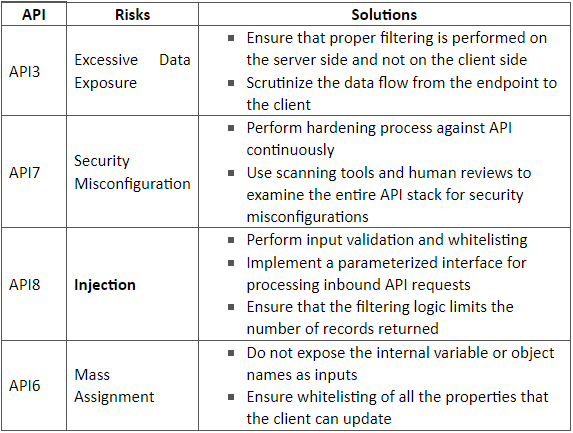
\includegraphics{exam_prep/API Security Risks.png}
    \item Fuzzing: Fuzzing: Attackers use the fuzzing technique to repeatedly send some random input to the target API to generate error messages that reveal critical information. To perform fuzzing, attackers use automated scripts that send numerous requests with varying combinations of input parameters. Attackers use tools such as Fuzzapi to perform fuzzing on the target API
    \item Invalid Input Attacks: In some scenarios, fuzzing is difficult to perform due to its structure. In such cases, attackers will give invalid inputs to the API, such as sending text in place of numbers, sending numbers in place of text, sending a greater number of characters than expected, and sending null characters, etc., to extract sensitive information from unexpected system behavior and error messages. At the same time, attackers also manipulate the HTTP headers and values targeting both API logic and the HTTP protocol.
    \item Malicious Input Attacks: In the attack discussed above, attackers try to retrieve sensitive information from unexpected system behavior or error messages. A more dangerous attack is where the attackers inject malicious input directly to target both the API and its hosting infrastructure. To perform this attack, attackers employ malicious message parsers using XML.
    \item Login/Credential Stuffing Attacks: Attackers often target login and validating systems because attacks on these systems are difficult to detect and stop using typical API security solutions. Attackers perform login attacks or credential stuffing attacks to exploit password reuse across multiple platforms. Most users use the same passwords to access different web services
    \item API Vulnerabilities:
    \begin{itemize}
        \item Enumerated Resources:
        \begin{itemize}
            \item Design flaws can cause serious vulnerability, disclosing information through unauthenticated public API
            \item Allows attackers to guess user IDs easily, compromising the security of the user data.
        \end{itemize}
        \item RBAC Pivilege Escalation: 
        \begin{itemize}
            \item Privilege escalation is a common vulnerability present in APIs having role-based access control (RBAC) where changes to endpoints are made without proper attention.
            \item Allow attackers to gain access to users' sensitive information.
        \end{itemize}
        \item No ABAC Validation:
        \begin{itemize}
            \item No proper attribute-based access control (ABAC) validation allows attackers to gain unauthorized access to API objects or perform actions such as viewing, updating, or deleting.
        \end{itemize}
        \item Buisness Logic Flaws:
        \begin{itemize}
            \item Many APIs come with vulnerabilities in buisness logic.
            \item Allows attackers to exploit legitimate workflows for malicious purposes.
        \end{itemize}
    \end{itemize}
\end{itemize}
\subsubsection{Web App Security}
\begin{itemize}
    \item Countermeasures for Watering Hole Attack:
    \begin{itemize}
        \item Apply software patches regularly to remove any vulnerabilities
        \item Monitor network traffic
        \item Secure DNS server to prevent attackers from redirecting the site to a new location.
        \item Analyze user behavior
        \item Inspect popular websites
        \item Use browser blug-ins that block HTTP redirects
        \item Disable third-party content such as advertizing services, which track user activities.
        \item Make sure to hide online activities with a VPN and enable the browser's private browsing feature.
        \item Make sure to run the web browser in a virtual environment to limit access to local system.
    \end{itemize}
    \item Countermeasures against command injection flaws are:
    \begin{itemize}
        \item Perform input validation
        \item Escape dangerous characters
        \item Use language-specific libraries that avoid problems due to shell commands
        \item Perform input and output encoding
        \item Use a safe API that avoids use of the interpreter entirely
        \item Structure requests so that all supplied parameters are treated as data rather than potentially executable content
        \item Use parameterized SQL queries
        \item Use modular shell disassociation from the kernel
        \item Use built-in library functions and avoid calling OS commands directly
    \end{itemize}
    \item countermeasures to defend broken authentication and session management attacks include:
    \begin{itemize}
        \item Use SSL for all authenticated parts of the application
        \item Verify whether all the users' identities and credentials are stored in a hashed form
        \item Never submit session data as part of a GET, POST
        \item Apply pass phrasing with at least five random words
        \item Limit the login attempts and lock the account for a specific period after a certain number of failed attempts
        \item Use a secure platform session manager to generate long random session identifiers for secure session development
        \item Make sure to check weak passwords against a list of the top bad passwords
    \end{itemize}
    \item Countermeasures to defend against broken access control:
    \begin{itemize}
        \item Perform access control checks before redirecting the authorized user to the requested resource
        \item Avoid using insecure IDs to prevent the attacker from guessing them
        \item Implement a session timeout mechanism
        \item Limit file permissions to authorized users to avoid misuse
        \item Avoid client-side caching mechanisms
        \item Remove session tokens on the server side on user logout
        \item Ensure that minimum privileges are assigned to users to perform only essential actions
        \item Enforce access control mechanisms once and re-use them throughout the application
    \end{itemize}
    \item Cookies flagged as secure are only transmitted over HTTPS
    \item Fuzz testing: Web application Fuzz testing (fuzzing) is a black box testing method. It is quality checking and assurance technique used to identify coding errors and security loopholes in web applications. Huge amounts of random data called "fuzz" is generated by the fuzz testing tools (fuzzers) and used against the target web application to discover vulnerabilities that can be exploited by various attacks.
    \begin{itemize}
        \item Mutation-based: current data samples create new test data and the new test data again mutates to generate further random data. This type of testin starts with a valid sample and keeps mutating until the target is reached.
        \item Protocol-Based: protocol fuzzer send forged packets to the target application that is to be tested
        \item Generation-Based
    \end{itemize}
\end{itemize}

\subsection{SQL Injection}
\subsubsection{SQL Injection Concpets}
\begin{itemize}
    \item Types of attacks:
    \begin{itemize}
        \item Authorization Bypass: Using this attack, an attacker alters authorization information stored in the database by exploiting an SQL injection vulnerability.
        \item Compromised Data Integrity: Using this attack, an attacker defaces a web page, inserts malicious content into web pages, or alters the contents of a database.
        \item Remote Code Execution: Using this attack, an attacker compromises the host OS.
        \item Compromised Availability of Data: Using this attack, an attacker deletes the database information, delete logs, or audit information stored in a database.
    \end{itemize}
\end{itemize}
\subsubsection{Types of SQL Injection}
\begin{itemize}
    \item Union SQL Injection: In a UNION SQL injection, an attacker combines a forged query with a query requested by the user using a UNION clause.
    \item Blind/Inferential SQL Injection: In blind SQL injection, an attacker poses a true or false question to the database to determine whether the application is vulnerable to SQL injection.
    \item Error-based SQL injection: In this type of SQL injection, the attacker forces the database to return error messages in response to his/her inputs. Later, the attacker may analyze the error messages obtained from the underlying database to gather information that can be used for constructing the malicious query.
    \item In-band SQL injection: In in-band SQL injection, attackers use the same communication channel to perform the attack and retrieve the results.
    \item Out-of-band SQL Injection: Attacker uses different communication channels to perform the attack and obtain results. Difficult to perform as the attacker needs to communicate with a database server and determine the server features used by a web application.
    \item tautology-based SQL injection attack, an attacker uses a conditional OR clause in such a way that the condition of the WHERE clause will always be true.
    \item end-of-line SQL injection, an attacker uses Line comments in specific SQL injection inputs.
    \item Piggybacked Query: Attacker injects an additional malicious query into the original query.
\end{itemize}
\subsubsection{SQL Injection Methodology}
\begin{itemize}
    \item Database Objects:
    \begin{itemize}
        \item Oracle:
        \begin{itemize}
            \item SYS.USER\_OBJECTS
            \item SYS.TABLES, SYS.USER\_TABLES
            \item SYS.USER\_VIEWS
            \item SYS.ALL\_TABLES
            \item SYS.COLUMNS
            \item SYS.USER\_OBJECTS
        \end{itemize}
        \item MS Access
        \begin{itemize}
            \item MsysACEs
            \item MsysObjects
            \item MsysQueries
            \item MsysRelationships
        \end{itemize}
        \item MySQL:
        \begin{itemize}
            \item mysql.user
            \item mysql.db
            \item mysql.tables\_priv
        \end{itemize}
        \item MSSQL Server:
        \begin{itemize}
            \item sysobjects
            \item syscolumns
            \item systypes
            \item sysdatabases
        \end{itemize}
        \item DB2:
        \begin{itemize}
            \item syscat.columns
        \end{itemize}
    \end{itemize}
    \item Functions:
    \begin{itemize}
        \item LOAD\_FILE(): function within MySQL and is used to read and return the contents of a file located within MySQL server.
        \item OPENROWSET(): An SQL Server can be linked back to an attacker's DB via OPENROWSET.
        \item CONVERT(): Used to convert one data type to another.
        \item INTO OUTFILE(): The OUTFILE function within MySQL is often used to run a query and dump the results into a file.
        \item CHAR(): attacker can encode a common injection variable present in the input string in an attempt to avoid detection in the signatures of network security measures. Converts hexadecimal values into characters that can easily pass through SQL engine parsing. For MySQL.
        \item ASCIISTR(): Oracle function that takes a string (or an expression that resolves to a string), and returns an ASCII version of the string in the cur.
        \item CHR(): Oracle function that returns the ASCII character that corresponds to the value passed to it.
    \end{itemize}
    \item Column Enumeration:
    \begin{itemize}
        \item MSSQL:\\
        \verb|SELECT name FROM syscolumns WHERE id = (SELECT id FROM sysobjects WHERE name = 'tablename')sp_columns tablename|
        \item MySQL:\\
        \verb|show columns from tablename|
        \item Oracle:
        \verb|SELECT * FROM all_tab_columns WHERE table_name='tablename'|
        \item DB2:\\
        SELECT * FROM syscat.columns WHERE tabname='tablename'|
    \end{itemize}
    \item single and double quotes: In black box testing, single and double quotes are used as the input data to catch instances where the user input is not sanatized.
    \item Semicolon: In black box penetration testing, a semicolon is used to group two or more SQL statements in the same line.
    \item Static Code analysis: Main objective is to improve the quality of software products by finding errors in the early stages of the development lifecycle. Code is not executed. Covers structural and statement coverage testing.
    \item Dynamic code analysis: Checks for functional behavior of the software system, memory/CPU usage, and overall performance of the system. In dynamic testing code is executed to uncover bugs in the software system. Testing is done in the later stages of the software development lifecycle.
    \item Variations: Uses the WHERE statement that always evaluates to true, so that any mathematical or string comparison can be used. It is performed by placing characters such as \verb|' or '1'='1'| on any basic injection statement.
    \item Declare Variables: uses variables that can be used to pass a series of specially crafted SQL statements and bypass the detection mechanism.
    \item Case Variation: Obfuscate an SQL statement by mixing it with uppercase and lowercase letters.
    \item Null Byte: Uses the null byte (\verb|%00|) character prior to a string in order to bypass the detection mechanism.
\end{itemize}
\subsubsection{SQL Injection Countermeasures}
\begin{itemize}
    \item Tools:
    \begin{itemize}
        \item Acunetix Web Vulnerability Scanner provides automated web application security testing with innovative technologies including DeepScan and AcuSensor Technology. Rigorously tests for thousands of web application vulnerabilities including SQL injeciton and XSS.
    \end{itemize}
\end{itemize}


\subsection{Hacking Wireless Networks}
\subsubsection{Wireless Concepts}
\begin{itemize}
    \item Orthogonal Frequency-division Multiplexing (OFDM): Method of encoding digital data on multiple carrier frequencies.
    \item Frequency-hopping Spread Spectrum (FHSS): A method of transmitting radio signals by rapidly switching a carrier among many frequency channels.
    \item Multiple input, multiple output orthogonal frequency-division multiplexing (MIMO-OFDM): An air interface for 4G and 5G broadband wireless communications.
    \item Direct-sequence Spread Spectrum (DSSS): An original data signal multiplied with a pseudo-random noise spreading the code.
    \item Shared Key authentication: each wireless station recieves a shared secret key over a secure channel that is distinct from the 802.11 wireless network communication channels. The following steps illustrate the establishment of connectino in the shared key authentication process
    \begin{itemize}
        \item Station sends an authentication frame to the AP.
        \item The AP sends a challenge text to the station.
        \item The station encrypts the challenge text by making use of its configured 64- or 128-bit key, and it sends the encrypted text to the AP.
        \item The AP uses its configured WEP key to decrypt the encrypted text. The AP compares the decrypted text with the original challenge text. If the decrypted text matches the original challenge text, the AP authenticates the station.
        \item The station connects to the network.
    \end{itemize}
    \item Wireless Standards:
    \begin{itemize}
        \item 802.11d: Enchanced version of 802.11a and 802.11b. Supports regulatory domains. The particulars of this standard can be set at the media access control (MAC) layer.
        \item 802.11e: Used for real-time applications such as voice, VoIP, and video. To ensure that these time-sensitive applications have the network resources they need, 802.11e defines mechanisms to ensure Quality of Service (QoS) to Layer 2 of the reference model, the medium-access layer, or MAC.
        \item 802.11i: Improves WLAN security by implementing new encryption protocols such as TKIP and AES. It is a standard for wireless local area networks (WLANs) that provides improved encryption for networks that use the popular 802.11a, 802.11b (which includes Wi-Fi) and 802.11g standards.
        \item 802.11n: A revision that enhances the earlier 802.11g standards with multiple-input multiple-output (MIMO) antennas. It works in both the 2.4GHz and 5GHz bands. IEEE industry standard for Wi-Fi wireless local network transportations. Digital Audio Broadcasting (DAB) and Wireless LAN use OFDM.
        \item IEEE 802.16: wireless communication standard designed to provide multiple physical layer (PHY) and media access control (MAC) options. It is also known as WiMax. This standard is a specification for fixed broadband wireless metropolitan access networks (MANs) that use point-to-multipoint architecture. It has a range of 1609.34-9656.06 Kilometers (1-6 miles).
    \end{itemize}
\end{itemize}
\subsubsection{Wireless Encryption}
\begin{itemize}
    \item PEEAP: a protocol that encapsulates the EAP within an encrypted and authenticated transport layer security (TLS) tunnel.
    \item WEP: An encryption algorithm for IEEE 802.11 wireless networks. Uses RC4 encryption with a 40/104-bit key. CRC-32 for integrity checking. Does not provide cryptographic integrity protection.
    \item CCMP: An encryption protocol used in WPA2 for strong encryption and authentication.
    \item WPA: RC4 and TKIP encryption algorithms with 128-bit keys. Michael algorithm and CRC-32 for integrity checking. Succeptable to KRACK.
    \item WPA2: An upgrade to WAP using AES and CCMP for wireless data encryption. Introduces the National Institute of Standards and Technology (NIST) FIPS 140-2-compliant AES encryption algorithm, a strong wireless encryption, and counter mode cipher block chaining message authentication code protocol (CCMP). Provides stronger data protection and network access control. Gives a high level of security to Wi-Fi connections, so that only authorized user can access it. 128-bit key, CBC-MAC for integrity checking.
    \item WPA3: Is a third generation Wi-Fi security protocol that provides new features for personal and enterprise usage. It uses Galois/Counter Mode-256 (GCMP-256) for encryption and the 384-bit hash message authentication code with the Secure Hash Algorithm (HMAC-SHA-384) for authentication. Susceptable to Dragonblood vulnerabilities.
    \item WPA: 
    \item Counter Mode Cipher Block Chaining Message Authentication Protocol (CCMP): an encryption protocol used in WPA2 for stronger encryption and authentication. Uses AES
\end{itemize}
\subsubsection{Wireless Threats}
\begin{itemize}
    \item Confidentiality Attack: Attempt to intercept confidential information sent over wireless associationsm regardless of whether they were sent in clear text or encrypted by Wi-Fi protocols.
    \item Availability Attacks: Aim at obstructing the delivery of wireless services to legitmiate users, wither by crippling those resources or by denying them access to WLAN resources.
    \item Authentication Attacks: Steal the identity of Wi-Fi clients, their personal infomration, login credentials, etc. to gain unauthorized access to network resources.
    \item Integrity Attacks: Attackers send forged control, management, or data frames over a wireless network to misdirect the wireless devices to perform anothe type of attacks (e.g., DoS).
    \item Ad hoc associations: An attacker may perform this kind of attack using any Universal Serial Bus (USB) adapter or wireless card. The attacker connects the host to an unsecured client to attack a specific client or to avoid AP security.
    \item Promiscuous Client: Allows an attacker to transmit target network traffic through a fake AP. It is very similar to the evil-twin threat on wireless networks, in which an attacker launches an AP that poses as an authorized AP by beaconing the WLAN's SSID.
    \item Client mis-associtaion: The client may intentionally or accidentally connect or associtae with an AP outside of the legitimate network because the WLAN signals travel through the air, walls, and othe obstructions.
    \item Unauthorized association: A major threat to wireless networks. The prevention of this kind of attack depends on the method or technique that the attacker uses to get associated with a network.
\end{itemize}
\subsubsection{Wireless Hacking Methodology}
\begin{itemize}
    \item Tools:
    \begin{itemize}
        \item Netcat: A networking utility that reads and writes data across network connections, using the TCP/IP protocol. It is a reliable "back-end" tool used directly or driven by othe programs and scripts. It is also a network debugging and exploration tool.
        \item NetStumbler: Used for collecting wireless packets and detecting wireless LANs using 802.11b, 802.11a and 802.11g WLAN standards. Runs on Windows.
        \item L0phtCrack: Tool designed to audit passwords and recover applications. Recovers lost Microsoft Windows passwords with the help of a dictionary, hybrid, rainbow table, and brute-force attacks, also checks the strenght of the password.
        \item Kismet: An 802.11 Layer 2 wireless network detector, sniffer, and intrusion detection system. Identifies networks by passively collecting packets and detecting standard named networks. It detects hidden networks and the presence of non-beaconing networks via traffic.
        \item Robber: Open-source tool that helps attackers to find executalbes prone to DLL hijacking. 
        \item CommView for WiFi: CommView for Wi-Fi is a wireless network monitor and analyzer for 802.11 a/b/g/n networks. It captures packets to display important information such as the list of APs and stations, per-node and per-channel statistics, signal strength, a list of packets and network connections, protocol distribution charts, etc. By providing this information, CommView for Wi-Fi can view and examine packets, pinpoint network problems, and troubleshoot software and hardware.
        \item WiFiFoFum: WiFiFoFum is a wardriving app to locate, display and map found WiFi networks. WiFiFoFum scans for 802.11 Wi-Fi networks and displays information about each including: SSID, MAC, RSSI, channel, and security. WiFiFoFum also allows you to connect to networks you find and log the location using the GPS. KML logs can be emailed.
        \item BlueScan: BlueScan is a bash script that implements a scanner to detect Bluetooth devices that are within the range of our system. BlueScan works in a non-intrusive way, that is, without establishing a connection with the devices found and without being detected. Superuser privileges are not necessary to execute it.
        \item  WiFish Finder: WiFish Finder is a tool for assessing whether WiFi devices active in the air are vulnerable to 'Wi-Fishing' attacks. Assessment is performed through a combination of passive traffic sniffing and active probing techniques. Most WiFi clients keep a memory of networks (SSIDs) they have connected to in the past. Wi-Fish Finder first builds a list of probed networks and then using a set of clever techniques also determines security setting of each probed network. A client is a fishing target if it is actively seeking to connect to an OPEN or a WEP network.
    \end{itemize}
    \item WarFlying: Attackers use drones to detect open wireless networks.
    \item WarWalking: Attackers walk around with Wi-Fi-enabled laptops installed with a wireless discovery tool to map out open wireless networks.
    \item WarDriving: Attacker drive around with WiFi enabled laptops installed with a wireless discovery tool to map out open wireless networks.
    \item WarChalking: Symbols are drawn in public places to advertise open Wi-Fi networks.
\end{itemize}
\subsubsection{Bluetooth Hacking}
\begin{itemize}
    \item Protocols:
    \begin{itemize}
        \item Link management protocol (LMP): Used for control of the radio link between two devices, handling matters such as link establishment, querying device abilities and power control. It is implemented on the controller.
        \item OBEX: Object Exchange protocol is used for communicating binary objects between devies. Bluejacking is sending anonymouse message to othe Bluetooth-equipped devices via the OBEX protocol
        \item Logical link control and adaptation protocol (L2CAP): L2CAP passes packets to either the Host Controller Interface (HCI) or on a hostless system, directly to the Link Manager/ACL link.
        \item Service Discovery Protocol (SDP): Is used to allow devices to discover what services each other support, and what parameters to use to connect to them.
    \end{itemize}
    \item Non-pairable mode: In the non-pairable mode, a Bluetooth device rejects pairing requests sent by any device.
    \item Limited discoverable mode: In the limited discoverable mode, the Bluetooth devices are discoverable only for a limited period, for a specific event, or during temporary conditions.
    \item Non-discoverable mode: Setting a Bluetooth device to the non-discoverable mode prevents that device from appearing on the list during a Bluetooth-enabled device search process. However, it remains visible to users and devices that were previously paired with it or know its MAC address.
    \item Discoverable mode: When Bluetooth devices are in the discoverable mode, they are visible to other Bluetooth-enabled devices. If a device attempts to connect to another, the device attempting to establish the connection must search for a device that is in the discoverable mode; otherwise, the device attempting to initiate the connection will not be able to detect the other device.
    \item BluePrinting: BluePrinting is a footprinting technique performed by an attacker in order to determine the make, device model, firmware version, etc. of the target Bluetooth-enabled device. Attackers collect such information from remote bluetooth devices and analyze them in an attempt to find out whether the devices are in the range of vulnerability to exploit.
    \item Bluejacking: Bluejacking is the use of Bluetooth to send messages to users without the recipient's consent, similar to email spamming. Prior to any Bluetooth communication, the device initiating connection must provide a name that is displayed on the recipient's screen. As this name is user-defined, it can be set to be an annoying message or advertisement. Strictly speaking, Bluejacking does not cause any damage to the receiving device. However, it may be irritating and disruptive to the victims. OBEX protocol.
    \item Bluebugging: Bluebugging is an attack in which an attacker gains remote access to a target Bluetooth-enabled device without the victim being aware of it. In this attack, an attacker sniffs sensitive information and might perform malicious activities such as intercepting phone calls and messages, forwarding calls and text messages, etc.
    \item BlueSniff: BlueSniff is a proof of concept code for a Bluetooth wardriving utility. It is useful for finding hidden and discoverable Bluetooth devices. It operates on Linux.
\end{itemize}
\subsubsection{Wireless Security Tools and Hacking Countermeasures}
\begin{itemize}
    \item Countermeasures to prevent KRACK attacks:
    \begin{itemize}
        \item Update all the routers and Wi-Fi devices with the latest security patches.
        \item Turn on auto updates for all the wireless devices and patch the device firmware.
        \item Avoid using public Wi-Fi networks.
        \item Browse only secured websites and do not access sensitive resources when the device is connected to an unprotected network.
        \item If there are IoT devices, audit the devices and do not connect to insecure Wi-Fi routers.
        \item Always enable the HTTPS Everywhere extension.
        \item Enable two-factor authentication.
        \item Use a VPN to secure information in transit.
    \end{itemize}
    \item SSID Cloaking: Used to keep default wireless messages from broadcasting the ID to everyone.
    \item RF Scanning: Re-purposed access points that do only packet capturing and analysis (RF sensors) are plugged in all over the wired network to detect and warn the WLAN administrator about any wireless devices operating in the area.
    \item Wired Side Inputs: Network management software uses this technique to detect rogue APs. This software detects devices connected in the LAN, including Telnet, SNMP, CDP (Cisco discovery protocol) using multiple protocols.
    \item AP Scanning: Access points that have the functionality of detecting neighboring APs operating in the nearby area will expose the data through its MIBS and web interface.
    \item Wireless control system: Provides the means to configure the wireless IPS service on the MSE, push wireless IPS configurations to the controller, and set APs in the wireless IPS monitor mode.
    \item Wireless LAN controller(s): These controllers forward attack information from wireless IPS monitor-mode APs to the MSE and distributes configuration parameters to Aps.
    \item Mobility services engine: It is the central point of alarm aggregation from all controllers and their respective wireless IPS monitor-mode APs. Alarm information and forensic files are stored on the system for archival.
    \item  Local mode AP: This mode provides wireless service to clients in addition to time-sliced rogue and location scanning.
\end{itemize}

\subsection{Hacking Mobile Platforms}
\subsubsection{Mobile Platform Attack Vectors}
\begin{itemize}
    \item M1 - Improper Platform Usage: This category covers the misuse of a platform feature or the failure to use platform security controls. It includes Android intents, platform permissions, and the misuse of Touch ID, Keychain, or some other security control that is part of the mobile device's OS
    \item M3 - Insecure Communication: This category covers poor handshaking, incorrect SSL versions, weak negotiation, cleartext communication of sensitive assets, and so on. Such flaws expose an individual user's data and can lead to account theft.
    \item M7 - Client Code Quality: This category covers "Security Decisions via Untrusted Inputs" and is one of the less frequently used categories. it is the catch-all for code-level implementation problems in the mobile client, which are distinct from server-side coding mistakes.
    \item M8 - Code Tampering: This category covers binary patching, local resource modification, method hooking, method swizzling, and dynamic memory modification.
\end{itemize}
\subsubsection{Hacking Android OS}
\begin{itemize}
    \item Countermeasures that can help you to protect your Android device and the data stored on it from malicious users.
    \begin{itemize}
        \item Enable screen lock for your phone.
        \item Never root your android device.
        \item Download apps only from official Android markets
        \item Keep your device updated with Google Android anti-virus software.
        \item Do not directly download APKs
        \item Update the OS regularly
        \item Use a free protector Android apps such as Android Protector, where you can assigne passwords to text messages, mail accounts, and so on.
        \item Customize your locked home screen with the user information.
        \item Enable encryption in your Android device to enhance its security.
        \item Lock your apps that hold private information to prevent other from viewing it, using apps such as AppLock.
        \item Enable GPS on your Android device for it to be tracked when lost or stolen.
        \item Enable two-step verification on your Android mobile device.
        \item Never root your Android device
        \item Download apps only from official Android markets
        \item Uninstall apps that invade your privacy
        \item Encrypt all the Internet traffic through VPN services such as ExpressVPN and VyprVPN for Android.
        \item Block all the ads displayed by apps
        \item Enable two-step verification on your Android mobile device
        \item Disable features such as SmartLock instead of passwords, and auto sign-in functionality.
        \item Install password manager apps such as LastPass to manage passwords securely
        \item Enable the screen pinning option to securely access Android apps
    \end{itemize}
    \item Native libraries
    \begin{itemize}
        \item Open Max AL: Companion API to OpenGL ES but used for multimedia (video and audio) rather than audio only.
        \item Libc: Comprises System C libraries
        \item FreeType: Meant for rendering fonts.
        \item Surface Manager: Meant for display management.
        \item SSL: meant for Internet security.
        \item Open GL | ES: 2D and 3D graphics library
        \item WebKit and Blink: Web browser engine to display HTML content.
        \item SQLite: database engine used for data storage purposes.
    \end{itemize}
    \item Storage:
    \begin{itemize}
        \item Shared Preferences: Stores private parameters in key values pairs
        \item Internal Storage: Private data on the deivce
        \item External Storage: Public data on the shared external storage
        \item SQLite Databases: Store structed data in a private database.
    \end{itemize}
    \item Tools:
    \begin{itemize}
        \item zANTI: android application which allows you to perform various attacks.
        \item LOIC Low orbit ion cannon: mobile application that allows the attacker to perform DoS/DDoS attacks on the target IP address.
        \item DroidSheep: simple Android tool for web session hacking (sidejacking).
        \item TunesGo is an Android tool that has an advanced android root module that recognizes and analyzes your Android device and chooses the appropriate Android root plan for it automatically.
        \item Orbot: proxy app that empowers other apps to use the internet more privately. Uses Tor to encrypt internet traffic and then hides it by bouncing through a series of computers around the world.
        \item NetCut: Allows attackers to identify the target devices and block the access of Wi-Fi to the victim devices in a network.
        \item X-Ray: Android vulnerability scanning tool.
    \end{itemize}
\end{itemize}
\subsubsection{Hacking iOS}
\begin{itemize}
    \item Apricot: Web-based mirror operating system for all the latest iPhones
    \item Spyzie: attackers use various online tools such as Spyzie to hack the target iOS mobile devices. Allows attacker to hack SMS, call logs, app chats, GPS, etc.
    \item Cydia: Software application for iOS that enables a user to find and install software packages on a jailbroken iPhone.
    \item Hexxa Plus: a jailbreak repo extractor for iOS 13.2 which allows you to install themes, tweaks, and apps. Compatible with iOS 13, up to 13.2.3.
    \item xHelper: Android/Trojan.Dropper.xHelper is a variant of Android/Trojan.Dopper. The first noticeable characteristic of xHelper is the use of stolen package names. For Instance, xHelper uses package names starting with "com.muf". This package name is associated with a number of puzzle names found on Google Play, including a puzzle called New2048HD with the package name com.mufc.fireuvw.
    \item Trident: A sophisticated spyware that exploits vulnerabilities in an iPhone to spy on users. These vulnerabilities allow attackers to jailbreak the target iPhone remotely and install malicious spyware such as Pegasus. Trident is capable of taking complete control of the target mobile device, and it allows attackers to monitor and track all the user activities.
    \item Gustuff: A type of banking trojan that uses malicious SMS to compromise the security of the target Android mobile device.
    \item iOS layers:
    \begin{itemize}
        \item Cocoa Application: This layer contains key frameworks that help in building iOS apps. These frameworks define the appearance of the apps, offer basic app infrastructure, and support key technologies such as multitasking, touch-based input, push notifications, and many high-level system services. Cocoa apps use the AppKit framework.
        \item Media: This layer contains the graphics, audio, and video technologies that enable multimedia experiences in apps.
        \item Core OS: This layer contains low-level features on which most other technologies are based. Frameworks in this layer are useful when dealing explicitly with security or communicating with an external hardware and networks. The services provided by this layer are dependent on the Kernel and Device Drivers layer
        \item Core Services: This layer contains fundamental system services for apps. The key services are Core Foundation and Foundation frameworks (define the basic types that all apps use). Individual technologies that support features such as social media, iCloud, location, and networking belong to this layer
    \end{itemize}
    \item untethered jailbreak: If the user turns the device off and back on, the device will start up completely, and the kernel will be patched without the help of a computer - it will be jailbroken after each reboot.
    \item semi-tethered jailbreak: has the property that if the user turns the device off and back on, the device will start up completely; it will no longer have a patched kernel, but it will still be usable for normal functions. To use jailbroken addons, the user needs to start the device with the help of the jailbreaking tool.
    \item iOS jailbreaking tools:
    \begin{itemize}
        \item Yalu
        \item Velonzy
        \item TaiG
    \end{itemize}
    \item Unrevoked: Android Jailbreaking tool.
    \item Userland Exploit: uses a loophole in the system application. It allows user-level access but does not allow iboot-level access. you cannot secure iOS devices against this exploit, as nothing can cause a recovery mode loop. Only firmware updates can patch these types of vulnerabilities. iBoot Exploit and Bootrom Exploit allow user-level access and also iboot-level access.
\end{itemize}
\subsubsection{Mobile Devices Management}
\begin{itemize}
    \item Tools:
    \begin{itemize}
        \item XenMobile: Complete Mobile device management software
        \item SpyBubble: Geolocation tracking
        \item Phonty: Geolocation tracking
        \item GadgetTrak: Geolocation tracking
    \end{itemize}
\end{itemize}
\subsubsection{Mobile Security Guidelines and Tools}
\begin{itemize}
    \item Tools:
    \begin{itemize}
        \item Promon Shield: Promon SHIELD is used to protect mobile apps against repackaging attacks. It detects when an app has been modified (repackaged). Consequently, the original app that has Promon SHIELD™ implemented cannot be executed when repackaged
        \item Lookout Personal: Lookout Personal helps to protect your device from security threats, loss, and theft. It is available for Android and iOS devices. It provides mobile security, identity protection, and theft prevention in a single app
        \item Apktool: Apktool is used for reverse engineering third-party, closed, binary Android apps. It can decode resources nearly to their original form and rebuild them after making some modifications. It also makes working with an app easier because of the project-like file structure and automation of some repetitive tasks such as building APK, etc
        \item FaceNiff: FaceNiff is an Android app that can sniff and intercept web session profiles over a Wi-Fi connection to a mobile.
    \end{itemize}
\end{itemize}

\subsection{IoT and OT Hacking}
\subsubsection{IoT Concepts}
\begin{itemize}
    \item Layers
    \begin{itemize}
        \item Internet Layer: A crucial layer as it servers as the main component in carrying out communication between two endpoints, such as device-to-device, device-to-cloud, device-to-gateway, or back-end data sharing.
        \item Access Gateway Layer: This layer helps to bridge the gap between two endpoints, such as a device and a client. The initial data handling also takes place in this layer. This layer carries out message routing, message identification, and subscribing.
        \item Middleware Layer: This is one of the most critical layers that operates in two-way mode. It is responsible for important functions such as data management, device management, and various issues like data analysis, data aggregation, data filtering, device information discovery, and access control.
        \item Edge Technology Layer: This layer consists of all the hardware components, including sensors, radio-frequency identification (RFID) tags, readers, or other soft sensors, and the device itself.
        \item Application Layer: This layer is placed at the top of the stack, is responsible for the delivery of services the the respective users from different sectors like building, industrial, manufacturing, automobile, security, healthcare, etc.
    \end{itemize}
    \item Communication Protocol:
    \begin{itemize}
        \item Very Small Aperture Terminal (VSAT): A communication protocol that is used for data transfer using small dish antennas for both broadband and narrowband data.
        \item QUIC: Quick UDP Internet Connections (QUICs) are multiplexed connection between IoT devices over the User Datagram Protocol (UDP); they provide security equivalent to SSL/TLS.
        \item Near-Field Communication (NFC): NFC is a type of short-range communication that uses magnetic field induction to enable communication between two electronic devices. It is primarily used in contactless mobile payment, social networking, and the indentifiaction of documents or other products.
        \item Power-Line Communication (PLC): This is a type of protocol that uses electrical wire to transmit power and data from one endpoint to another. PLC is required for applications in deffernt areas such as home automation, industrial devices, and broadband over power lines (BPL).
        \item Constrained Application Protocol (CoAP): A web transfer protocol used to transfer messages between constrained nodes and IoT networks.
        \item LWM2M: Lightweight Machine-to-Machine (LWM2M): An application-layer communication protocol used for application-level communication between IoT devices.
        \item XMPP: eXtensible Messaging and Presence Protocol (XMPP) is an open technology for real-time communication used for IoT devices. This technology is used for developing interoperable devices, applications, and services for the IoT environment.
        \item Physical Web: technology used to enable faster and seamless interation with nearby IoT devices. It reveals the list of URLs being broadcast by nearby devices with BLE beacons.
    \end{itemize}
    \item Contiki: Used in low power wireless devices such as street lighting, sound monitoring systems, etc.
    \item Edge: Edge computing helps the IoT environment to move computational processing to the edge of the network, allowing smart devices and gateways to perform tasks and services from the cloud end.
    \item Sensing Technology: Sensors embedded in the devices sense a wide variety of informaition from their surroundings like temperature, gases, location, working of some industrial machine as well as sensing health data of a patient.
    \item IoT Gateways: Gateways are used to bridge the gap between the IoT devices (internal network) and the end user (external network) and thus allowing them to connect and communicate with each other. The data collected by the sensors in IoT devices send the collected data to the concerned user or cloud through the gateway.
    \item Cloud Server/Data storage: the collected data after travelling through the gateway arrives at the cloud, where it is stored and undergoes data analysis. The processed data is then transmitted to the user where he/she takes certain action based on the information recieved by him/her.
    \item Remote Control using Mobile App: The end user uses remote controls such as mobile phones, tabs, laptops, etc. installed with a mobile app to monitor, control, retrieve data, and take a specific action on IoT devices from a remote location.
\end{itemize}
\subsection{IoT Attacks}
\begin{itemize}
    \item Security issues at IoT layers:
    \begin{itemize}
        \item Cloud: Improper authentication, no encryption for storage and communications, insecure web interface.
        \item Mobile: Insecure API, lack of communication channels encryption, authenticationm lack of storage security.
        \item Network: Firewall, improper communications encryption, services, lack of automatic updates.
        \item Application: Validation of the inputted string, AuthN, AuthZ, no automatic security updates, default passwords.
    \end{itemize}
    \item Insecure Data Transfer and Storage: Lack of encryption and access control of data that is in transit or at rest may result in leakage of sensitive information to malicious users.
    \item Insecure Network Services: Prone to various attacks like buffer overflow attacks, which cause a denial-of-service scenario, thus leaving the device inaccessible to the user.
    \item Insecure Ecosystem Interfaces: Web, backend API, mobile, and cloud interfaces outside the devices lead to compromized security of the device and its components.
    \item Insecure Default settings: Insecure or insufficient device settings restrict the operators from modifying configurations to make the device more secure.
    \item Device Physical interface vulnerabilities:
    \begin{itemize}
        \item Firmware extraction
        \item User/Admin CLI
        \item Privileged escalation
        \item Reset to insecure state
        \item Removal of storage media
        \item Tamper resistance
        \item Debug port: UART (Serial), JTAG/SWD
        \item Device ID/serial number exposure.
    \end{itemize}
    \item Device Web Interface Vulnerabilities:
    \begin{itemize}
        \item Standard set of web application Vulnerabilities:
        \begin{itemize}
            \item OWASP Web Top 10
            \item OWASP ASVS
            \item OWASP Testing Guide
        \end{itemize}
        \item Credential management vulnerabilities
        \item Username enumeration
        \item Weak passwords
        \item account lockout
        \item Known default credentials
        \item insecure password recovery mechanism
    \end{itemize}
    \item Device Firmware Vulnerabilities:
    \begin{itemize}
        \item Sensitive data exposure (See OWASP Top 10 - A6 Sensitive data exposure):
        \begin{itemize}
            \item Backdoor accounts
            \item Hardcoded credentials
            \item Encryption keys
            \item Encryption (symmetric, asymmetric)
            \item sensitive infomration
            \item sensitive URL disclosure
        \end{itemize}
        \item Firmware version display and/or date of last update.
        \item Vulnerable services (web, ssh, tftp, etc.)
        \begin{itemize}
            \item Verify for old software versions and possible attacks (Heartbleed, Shellshock, old PHP versions, etc.)
        \end{itemize}
        \item Security-related function API exposure
        \item Firmware downgrade possibility
    \end{itemize}
    \item Network Traffic Vulnerabilities:
    \begin{itemize}
        \item LAN
        \item LAN to internet.
        \item Short range
        \item Non-standard
        \item Wireless (Wi-Fi, Z-wave, XBee, Zigbee, bluetooth, LoRa)
        \item Protocol fuzzing.
    \end{itemize}
    \item Sybil Attack: The attacker uses multiple forged identities to create a strong illusion of traffic congestion, affecting communication between neighboring nodes and networks.
    \item Exploitation Kits: The attacker uses malicious scripts to exploit poorly patched vulnerabilities in an IoT device.
    \item Side-Channel Attack: the attackeer extracts information about encryption keys by observing the emission of signals i.e. "side channels" from IoT devices.
    \item DNS Rebinding Attack: DNS rebinding is a process of obtaining access to a victim's router using a malicious JavaScript code on a web page.
    \item Hex Code: A color hex code is a way of specifying color using hexadecimal values. the code itself is a hex triplet, which represents three separate values that specify the levels of the component colors. It is used by programmers to describe locations in memory because it can represent every byte.
    \item Unicode: Character encoding system to support worldwide interchange, processing, and display of the written texts. This type of code is mostly used in evading IDS.
    \item Rolling Code: the form of a code from a modern key fob that locks or unlocks the vehicle. Here a code is sent to the vehicle which is defferent for every other use and is only used once, that means if a vehicle receives the same code again it rejects it. This code which locks or unlocks a car or garage is called as Rolling code or Hopping code. it is used in keyless entry systems to prevent replay attacks. An eavesdropper can capture the code transmitted and later use it to unlock the garage or vehicle.
    \item Polymorphic code: Code that uses a polymorphic engine to mutate while keeping the original algorithm intact. Polymorphic code can also be used to generate encryption algorithms.
\end{itemize}
\subsection{IoT Hacking Methodology}
\begin{itemize}
    \item Phases:
    \begin{itemize}
        \item Information Gathering
        \item Vulnerability Scanning
        \item Launching Attacks
        \item Gaining Remote Access
        \item Maintaining Remote Access
    \end{itemize}
    \item Tools:
    \begin{itemize}
        \item MultiPing: find the IP address of any IoT device in the target network.
        \item RFCrack: Attackers use RFCrack to obtain the rolling code sent by the victim to unlock a vehicle and later use the same code for unlocking and stealing the vehicle.
        \item FCC ID Search: Helps in finding the details and granted certification of devices. FCC ID contains two elements: Grantee ID (initial 3 or 5 characters) and Product ID (Remaining characters).
        \item IoT Seeker: will scan a network for specific types of IoT devices to detect if they are using the default, factory set credentials.
        \item Censys: A public search engine and data-processing facility backed by data collected from ongoing Internet-wide scans. Suports full-text searches on protocol banners and queries a wide range of derived fields. It can identify specific vulnerable devices and networks, and generate statistical reports on broad useage patterns and trends.
        \item RIoT: Vulnerability Scanner: Retina IoT identifies at-risk IoT devices, such as IP cameras, DVRs, printers, and routers. This tool gives an attacker's view of all the IoT devices and their associated vulnerabilities.
        \item Foren6: uses sniffers to capture 6LoWPAN traffic and renders the network state in a graphical user interface. Captures all RPL-related information and identifies abnormal behaviors.
        \item Zigbee Framework: Attify ZigBee framework consists of a set of tools used to perform ZigBee penetration testing. ZigBee protocol makes use of 16 different channels for all communications. Attackers use Zbstumbler from Attify Zigbee framework to identify the channel used by the target device.
        \item HackRF One: Attackers use HackRF One to perform attacks such as BlueBorne or AirBorne attacks such as replay, fuzzing, jamming, etc. HackRF One is an advanced hardware and software defined radio with the range of 1MHz to 6GHz. It transmits and receives radio waves in half-duplex mode, so it is easy for attackers to perform attacks using this device.
        \item Smartpage: Meta search engine
        \item MetaGer: Meta search engine
        \item eTools.ch: Meta search engine
        \item Thingful: Search engine for finding and using open IoT data from around the world. Helps organizations make better decisions with external IoT data.
        \item beSTORM: smart fuzzer that detects buffer overflow vulnerabilities by automating and documenting the process of delivering corrupted inputs and watching for an unexpected response from the application
        \item RTL-SDR: hardware is available in the form of a USB dongle that can be used to capture active radio signals in the vicinity (an Internet connection is not mandatory).
        \item Universal Radio Hacker (URH): a software of investigating unknown wireless protocols used by various IoT devices.
    \end{itemize}
    \item firmware analysis steps
    \begin{itemize}
        \item Obtain firmware
        \item Analyze firmware
        \item Extract filesystem
        \item mount filesystem
        \item analyze filesystem content
        \item Emulate firmware for dynamic testing
    \end{itemize}
\end{itemize}
\subsection{IoT Countermeasures}
\begin{itemize}
    \item Lack of Secure Update Mechanism:
    \begin{itemize}
        \item Verify the source and integrity of updates
        \item Encrypt communication between endpoints
        \item Notify end-users of security updates
    \end{itemize}
    \item Lack of Physical Hardening:
    \begin{itemize}
        \item Set unique password for BIOS/firmware
        \item Configure device boot order to prevent unauthorized booting
        \item Minimize the external ports such as USB ports
    \end{itemize}
    \item Lack of Device Management:
    \begin{itemize}
        \item Blacklist malicious devices from suspicious sources.
        \item Validate all asset attributes.
        \item Secure decommissioning of devices.
    \end{itemize}
    \item Insecure default settings:
    \begin{itemize}
        \item Changee the default usernames and passwords.
        \item Custom modify the privacy and security settings.
        \item Disable remote access to IoT devices when not in use.
    \end{itemize}
    \item Insecure network services:
    \begin{itemize}
        \item Close open network ports
        \item disable UPnP
        \item Review network services for vulnerabilities.
    \end{itemize}
    \item Insecure Web Interface:
    \begin{itemize}
        \item Enable default credentials to be changed.
        \item Enbale the account lockout mechanism
        \item Conduct periodic assessment of web applications
    \end{itemize}
    \item Insufficient Authentication / Authorization:
    \begin{itemize}
        \item Implement secure password recovery mechanisms
        \item Use strong and complex passwords.
        \item Enable two-factor authentication
    \end{itemize}
    \item Lack of Transport Encryption / Integrity Verification:
    \begin{itemize}
        \item Encrypt communication between endpoints.
        \item Maintain SSL/TLS implementation
        \item Not to use proprietary encryption solutions.
    \end{itemize}
    \item Security Considerations:
    \begin{itemize}
        \item Mobile: An ideal framework for the mobile interface should include proper authentication mechanism for the user, account lockout mechanism after a certain number of failed attempts, local storage security, encrypted communication channels and the security of the data transmitted over the channel.
        \item Gateway: An ideal framework for the gateway should incorporate strong encryption techniques for secure communications between endpoints. Also, the authentication mechanism for the edge components should be as strong as any other component in the framework. Where ever possible the gateway should be designed in such a way that it authenticates multi-directionally to carry out trusted communication between the edge and the cloud. Automatic updates should also be provided to the device for countering vulnerabilities.
        \item Cloud Platform: A secure framework for the cloud component should include encrypted communications, strong authentication credentials, secure web interface, encrypted storage, automatic updates and so on.
        \item Edge: Framework consideration for edge would be proper communications and storage encryption, no default credentials, strong passwords, use latest up to date components and so on.
    \end{itemize}
    \item Tools:
    \begin{itemize}
        \item DigiCert IoT Security Solution: DigiCert Home and Consumer IoT Security Solutions protect private data and home networks while preventing unauthorized access using PKI-based security solutions for consumer IoT devices.
        \item SeaCat.io: SeaCat.io is a security-first SaaS technology to operate IoT products in a reliable, scalable and secure manner. It provides protection to end users, business, and data.
        \item Firmalyzer Enterprise: Firmalyzer enables device vendors and security professionals to perform automated security assessment on software that powers IoT devices (firmware) in order to identify configuration and application vulnerabilities. This tool notifies users about the vulnerabilities discovered and assists to mitigate those in a timely manner.
    \end{itemize}
\end{itemize}
\subsection{OT Concepts}
\begin{itemize}
    \item DCS: A Distributed Control System (DCS) is used to control production systems spread within the same gepgraphical location.
    \item BPCS: Basic Process Control System (BPCS) is responsible for performing process control and monitoring for industrial infrastructure.
    \item SIS: A safety instrumented System (SIS) is an automated control system designed to safeguard the manufactureing environment in case of any hazardous incident in industry.
    \item PLC: A programmable logic controller (PLC) is a small solid-state control computer where instructions can be customized to perform a specific task. PLC is a Operational Technology (OT) component.
    \item SCADA: Supervisory Control and Data Acquisition (SCADA) is a centralized supervisory control system that is used for controlling and monitoring industrial facilities and infrastructure.
    \item Purdue Model:
    \begin{itemize}
        \item Level 0 (physiacl process): In this level, the actual physical process is defined, and the product is manufactured.
        \begin{itemize}
            \item BACnet, EtherCat, CANopen, Crimson v3, DeviceNet, GE-SRTP, Zigbee, ISA/IEC 62443, ISA SP100, MELSEC-Q, MODBUS, Niagara Fox, Omron Fins, PCWorx, Profibus, Profinet, Sercos II, S7 Communications, WiMax.
        \end{itemize}
        \item Level 1 (basic controls/intelligent devices): Analyzation and alteration of the physical process can be done at this level. The operations in basic control include "start motors", "open valves", "move actuators", etc.
        \begin{itemize}
            \item BACnet, EtherCat, CANopen, Crimson v3, DeviceNet, GE-SRTP, Zigbee, ISA/IEC 62443, ISA SP100, MELSEC-Q, MODBUS, Niagara Fox, Omron Fins, PCWorx, Profibus, Profinet, Sercos II, S7 Communications, WiMax.
        \end{itemize}
        \item Level 2 (Control Systems/Area Supervisory Controls): Supervising, monitoring, and controlling the physical process is carried out at this level.
        \begin{itemize}
            \item Level 2 uses protocols such as 6LoWPAN, DNP3, DNS/DNSSEC, FTE, HART-IP, IEC 60870-5-101/104, SOAP.
        \end{itemize}
        \item Level 3 (Operational Systems/Site Operations): In this level, the production management, individual plant monitoring, and control functions are defined.
        \item Level 4
        \begin{itemize}
            \item DCOM, DDE, FTP/SFTP, GE-SRTP, IPv4/IPv6, OPC, TCP/IP, Wi-Fi.
        \end{itemize}
        \item Level 5
        \begin{itemize}
            \item DCOM, DDE, FTP/SFTP, GE-SRTP, IPv4/IPv6, OPC, TCP/IP, Wi-Fi.
        \end{itemize}
    \end{itemize}
    \item ISA/IEC 62443: Provides a flexible framework for addressing and mitigating current and future security vulnerabilities in industrial automation and control systems.
    \item ICCP (IEC 60870-6): ICCP (inter-control center communications protocol) (IEC 68070) provides a set of standards and protocols for covering ICS or SCADA communication in power system automation.
    \item IEC 61850: A common protocol that enables interoperability and communications between the IEDs at electrical substations.
    \item HSCP: Hybrid SCP (Secure Copy Protocol): is developed for transmitting larger file sizes at high speed on long-distance and wideband infrastructure.
\end{itemize}
\subsection{OT Hacking Methodology and Countermeasures}
\begin{itemize}
    \item Tools:
    \begin{itemize}
        \item CRITIFENCE: Online tool that allows attackers to discover the default credentials of a device or product simply by entering the device name or manufacturer name
        \item GRASSMARLIN: Open source tool that passively maps and visually displays an ICS/SCADA network topology, while safely conducting device discovery, accounting and reporting on these critical cyber-physical systems.
        \item SCADA Shutdown tool: An ICS testing and automation tool that allows attackers to fuzz, scan, and run remote commands on ICSs, SCADA networks and controllers.
        \item Gqrx: An SDR implemented with the help of the GNU Radio and Qt GUI tool. Attackers use hardware devices such as FunCube dongles, Airspy, HackRF, and RTL-SDR along with Gqrx SDR, to analyze the spectrum.
    \end{itemize}
\end{itemize}

\subsection{Cloud Computing}
\subsubsection{Cloud Computing Concepts}
\begin{itemize}
    \item Cloud Deployment Models:
    \begin{itemize}
        \item Public Cloud: In this model, the provider makes services such as applications, servers, and data storage available to the public over the Internet. Therefore, he is liable for the creation and constant maintenance of the public cloud and its IT resources. Public cloud services may be free or based on a pay-per-usage model (e.g., Amazon Elastic Compute Cloud (EC2), Google App Engine, Windows Azure Services Platform, IBM Bluemix).
        \item Multi Cloud: It is a dynamic heterogeneous environment that combines workloads across multiple cloud vendors that are managed via one proprietary interface to achieve long-term business goals. The multi cloud uses multiple computing and storage services from different cloud vendors. It distributes cloud assets, software, applications, etc. across various cloud-hosting environments.
        \item Community Cloud: It is a multi-tenant infrastructure shared among organizations from a specific community with common computing concerns, such as security, regulatory compliance, performance requirements, and jurisdiction. The community cloud can be either on- or off-premises and governed by the participated organizations or by a third-party managed service provider (e.g., Optum Health Cloud, Salesforce Health Cloud).
        \item Hybrid Cloud: It is a cloud environment comprised of two or more clouds (private, public, or community) that remain unique entities but are bound together to offer the benefits of multiple deployment models. In this model, the organization makes available and manages some resources in-house and provides other resources externally (e.g., Microsoft Azure, Zymr, Parangat, Logicalis).
        \item Private Cloud: Internal or Corporate Cloud is a cloud infrastructure that a single organization operates solely. The organization can implement the private cloud within a corporate firewall. Organizations deploy private cloud infrastructures to retain full control over corporate data.
    \end{itemize}
    \item Cloud Storage Layers:
    \begin{itemize}
        \item Front-end layer: accessed by the end user where it provides APIs for the management of data storage.
        \item Middleware Layer: Performs several functions such as data de-duplication and replication of data.
        \item Back-end layer: Where the hardware is implemented.
        \item Application Layer: Is a cloud security control layer that includes software development lifecycle, binary analysis, scanners, web app firewalls, transactional sec, etc.
        \item 
    \end{itemize}
    \item NIST Cloud Deployment Actors:
    \begin{itemize}
        \item Cloud Carrier: Acts as an intermediary that provides connectivity and transport services between CSPs and cloud consumers. The cloud carrier provides access to consumers via a network, telecommunication, or other access devices.
        \item Cloud Auditor: A party that performs an independent examination of cloud service controls to express an opinion thereon. Audits verify adherence to standards through a review of the objective evidence.
        \item Cloud Consumer: A person or organization that maintains a business relationship with the cloud services providers (CSPs) and utilizes the cloud computing services.
        \item Cloud Provider: A person or organization who acquires and manages the computing infrastructure intended for providing services (directly or via a cloud broker) to interested parties via network access.
    \end{itemize}
    \item Infrastructure-as-a-service (IaaS): This cloud computing service enables subscribers to use on-demand fundamental IT resources, such as computing power, virtualization, data storage, and network. This service provides virtual machines and other abstracted hardware and operating systems (OSs), which may be controlled through a service application programming interface (API). As cloud service providers are responsible for managing the underlying cloud computing infrastructure, subscribers can avoid costs of human capital, hardware, and others (e.g., Amazon EC2, GoGrid, Microsoft OneDrive, Rackspace).
    \item Platform-as-a-Service (PaaS): This type of cloud computing service allows for the development of applications and services. Subscribers need not buy and manage the software and infrastructure underneath it but have authority over deployed applications and perhaps application hosting environment configurations. This offers development tools, configuration management, and deployment platforms on-demand, which can be used by subscribers to develop custom applications (e.g., Google App Engine, Salesforce, Microsoft Azure). Advantages of writing applications in the PaaS environment include dynamic scalability, automated backups, and other platform services, without the need to explicitly code for them.
    \item Software-as-a-Service (SaaS): This cloud computing service offers application software to subscribers on-demand over the Internet. The provider charges for the service on a pay-per-use basis, by subscription, by advertising, or by sharing among multiple users (e.g., web-based office applications like Google Docs or Calendar, Salesforce CRM, and Freshbooks).
    \item Identity-as-a-Service (IDaaS): This cloud computing service offers authentication services to the subscribed enterprises and is managed by a third-party vendor to provide identity and access management services. It provides services such as Single-Sign-On (SSO), Multi-Factor-Authentication (MFA), Identity Governance and Administration (IGA), access management, and intelligence collection. These services allow subscribers to access sensitive data more securely both on and off-premises (e.g., OneLogin, Centrify Identity Service, Microsoft Azure Active Directory, Okta).
    \item Anything-as-a-service (XaaS): also known as everything-as-a-service. Includes all the other types of cloud services.
    \item service Intermediation: Improves a given function by a specific capability and provides value-added services to cloud consumers.
    \item Service aggregation: Combines and integrates multiple services into one or more new services.
    \item Service Arbitrage: It is like service aggregation but without the fixing of the aggregated services (the cloud broker can choose services from multiple agencies).
    \item Distributed Storage: A characteristic of cloud computing that offers better scalability, availability, and reliability of data. However, cloud distributed storage can potentially raise security and compliance concerns.
    \item Automated Management: By minimizing user involvement, cloud automation speeds up the process and reduces labor costs and the possibility of human error.
    \item Measured Service: Cloud system employ the "pay-per-use" metering method. Subscribers pay for cloud services by monthly subscription or according to the usage of resources such as storage levels, processing power, and bandwidth. Cloud service providers monitor, control, report, and charge consumption of resources by customers with complete transparency.
    \item Virtualization Technology: Enables the rapid scaling of resources in a way that non-virtualized environments cannot achieve.
    \item Broad network access: Cloud resources are available over the network and accessed through standard procedures via a wide variety of platforms, including laptops, mobile phones, and personal digital assistants (PDAs).
    \item Rapid Elasticity: The cloud offers instant provisioning of capabilities to rapidly scale up or down, according to demand. To the consumers, the resources available for provisioning seem to be unlimited and can be purchased in any quantity at any point in time.
    \item Resource Pooling: Cloud service provider pools all the resources together to server multiple customers in the multi-tenant environment, with phtsical and virtual resources dynamically assigned and reassigned on demand by the consumer of the cloud.
\end{itemize}
\subsubsection{Container Technology and Serverless Computing}
\begin{itemize}
    \item Container Technology Tiers:
    \begin{itemize}
        \item Tier-1: Developer machines - image creation, testing and accreditation.
        \item Tier-2: Testing and accreditation systems - Verification and validation of image contents, signing images and sending them to the registries.
        \item Tier-3: Registries - Storing images and disseminating images to the orchestrators based on requests.
        \item Tier-4: Orchestrators - Transforming image into containers and deploying containers to hosts.
        \item Tier-5: Hosts - Operating and managing containers as instructed by the orchestrator.
    \end{itemize}
    \item Container network model:
    \begin{itemize}
        \item Sandbox: Comprises the container network stack configuration for the management of container interfaces, routing tables, and domain name system (DNS) settings.
        \item Endpoint: To maintain application portability, an endpoint is connected to a network and is abstracted away from the application, so that services can implement different network drives.
        \item Network Drivers: The network fucntions through the implementation of Docker network drivers. These drivers are pluggable so that multiple network drivers can be used concurrently on the same network. There are two types of CNM network drivers: namely native and remote network drivers.
        \item IPAM Drivers: IP address management (IPAM) drivers assign default subnet and IP addresses to the endpoints and networks if they are not assigned.
        \item Container Orchestration: an automated process of managing the lifecycles of software containers and their dynamic environments. It is used for scheduling and distributing the work of individual containers for microservices-based applications spread across multiple clusters.
        \item Bridge: A component of docker native network drivers. A bridge driver is used to create a Linux bridge on the host that is managed by the Docker.
        \item Network: A network is an interconnected collection of endpoints. Endpoints that do not have network connection cannot communicate over the network.
    \end{itemize}
    \item Docker netowrk drivers:
    \begin{itemize}
        \item Contiv: Open-source network plugin introduced by Cisco for building security and infrastructure policies for multi-tenant microservices deployments.
        \item Weave: Network plugin that is used to build a virtual network for connecting Docker containers spread across multiple clouds.
        \item Kuryr: A network plugin that implements the Docker libnetwork remote driver by using Neutron, an OpenStack networking service, and also includes a IPAM driver.
        \item MACVLAN: used to create a network connection between container interfaces and the parent host interface or sub-interfaces using the Linux MACVLAN bridge mode. It is a native network driver of a Docker engine.
        \item Host: By using a host driver, a container implements the host networking stack.
        \item Overlay: An overlay driver is used to enable container communication over the physical network infrastructure.
        \item None: A none driver implements its own networking stack and is isolated completely from the host networking stack.
    \end{itemize}
    \item Domain Snipping: Involves registering an elapsed domain name
    \item Microservices: Monolithic applications are broken down into cloud-hosted sub-applications called microservices that work together, each performing a unique task. As each microservice is packaged into the Docker container along with the required libraries, frameworks, and configuration files, microservices belonging to a single application can be developed and managed using multiple platforms.
    \item Docker Engine Components:
    \begin{itemize}
        \item Client CLI: the command line interface used to communicate with the daemon and where various Docker commands are initiated.
        \item Rest API: allows the communication and assignment of tasks to the daemon.
        \item Server: It is a persistent back-end process, also known as a daemon process (dockerd command).
        \item Docker Swarm: The Docker engine supports the swarm mode that allows managing multiple Docker engines within the Docker platform. Docker CLI is used for creating a swarm, deploying an application to the swarm, and handling its activity or behavior.
        \item Docker daemon: (dockerd) processes API requests and handles various Docker objects, such as containers, volumes, images, and networks.
        \item Docker images: Used to store and deploy containters. They are read-only binary templates with instructions for container creation.
        \item Docker registries: Locations where images are stored and pulled, and can be either private or public. Docker Cloud and Docker Hub are two popular public registries. Docker Hub is a predefined location of Docker images, which can be used by all users.
        \item Docker Client: The primary interface through which users communicate with Docker. When commands such as docker run are initiated, the client passes related commands to dockerd, which then executes them. Docker commands use the Docker API for communication.
    \end{itemize}
    \item Docker Objects:
    \begin{itemize}
        \item Images: Used to store and deploy containers. They are read-only binary templates with instructions for container creation.
        \item Services: Services enable users to extend the number of containers across daemons, and together they serve as a swarm with several managers and workers. Each swarm member is a daemon, and all these daemons can interact with each other using Docker API.
        \item Networking: is a channel through which all isolated containers communicate.
        \item Volumes: A storage where persisting data created by Docker and used by Docker containers are stored.
    \end{itemize}
    \item Kubernetes Architecture:
    \begin{itemize}
        \item Kube-proxy: A network proxy service that also runs on every worker node. This service maintains the network rules that enable network conncetion to the pods.
        \item Etcd cluster: A distributed and consistent key-value storage where Kubernetes cluster data, service discovery details, API objects, etc. are stored. It is a master node component.
        \item Container Runtime: A software designed to run the containers. Kubernetes supports various container runtimes, such as Docker, rktlet, containerd, and cri-o.
        \item Kubelet: Kubelet is an important service agent that runs on each node and ensures containers running in a pod. It also ensures pods and containers are healthy and running as expected. Kubelet does not handle containers that are not generated by Kubernetes.
    \end{itemize}
    \item Tools:
    \begin{itemize}
        \item Microsoft Azure Functions: 
        \item Knative
        \item Red Hat OpenShift
        \item Portainer
    \end{itemize}
\end{itemize}
\subsubsection{Cloud Computing Threats}
\begin{itemize}
    \item DNS Poisoning: Involves diverting users to a spoofed website by poisoning the DNS server or the DNS cache on the user's system.
    \item Cybersquatting: Involves conducting phishing scams by registering a domain name that is similar to a CSP.
    \item Domain Hijacking: Involves stealing a CSP domain name.
    \item Domain Snipping: Involves registering an elapsed domain name.
    \item Isolation failure: Multi-tenancy and shared resources are the characteristics of cloud computing. Strong isolation or compartmentalization of storage, memory, routing, and reputation among different tenants is lacking. Because of isolation failure, attackers try to control operations of other cloud customers to gain illegal access to the data.
    \item Privilege Escalation: A mistake in the access allocation system causes a customer, third party, or employee to get more access rights than needed.
    \item Illegal Access to the cloud: Attackers can exploit weak authentication and authorization to get illegal access, thereby compromising confidential and critical data stored in the cloud.
    \item Supply Chain Failure: A disruption in the chain may lead to loss of data privacy and integrity, unavailability of services, violation of SLA, economic and reputational losses resulting in failure to meet customer demand, and cascading failure.
    \item Abuse and Nefarious Use of Cloud services: Presence of weak registration systems in the cloud-computing environment gives rise to this threat. Attackers create anonymous access to cloud services and perpetrate various attacks such as password and critical cracking, building rainbow tables, CAPTCHA-solving farms, launching dynamic attack points, hosting exploits on cloud platforms, hosting malicious data, Botnet command or control, DDoS, etc.
    \item Insecure Interface and APIs: Attackers exploit user defined policies, reusable passwords/tokens, insufficient input-data validation.
    \item Data Breach/Loss: Attackers gain illegal access to the data and misuse or modify the data.
    \item Insufficient Due Diligence: Ignorance of CSP’s cloud environment poses risks in operational responsibilities such as security, encryption, incident response, and more issues such as contractual issues, design and architectural issues, etc.
    \item Session Hijacking Using Session Riding: Attackers exploit websites by engaging in cross-site request forgeries to transmit unauthorized commands. In session riding, attackers “ride” an active computer session by sending an email or tricking users to visit a malicious web page, during login, to an actual target site. When users click the malicious link, the website executes the request as if the user had already authenticated it. Commands used include modifying or deleting user data, performing online transactions, resetting passwords, and others.
    \item Wrapping Attack: It is performed during the translation of SOAP messages in the TLS layer, where attackers duplicate the body of the message and send it to the server as a legitimate user.
    \item DNS Attack: The attacker performs DNS attacks to obtain authentication credentials from Internet users.
    \item  Side Channel Attack: The attacker compromises the cloud by placing a malicious virtual machine near a target cloud server and then launches a side channel attack.
    \item Data remanence: Side channel attack
    \item Timing attack: side channel attack
    \item Acoustic cryptanalysis: side channel attack
\end{itemize}
\subsubsection{Cloud Hacking}
\begin{itemize}
    \item Tools:
    \begin{itemize}
        \item DumpsterDiver: autoamted tool to identify potential secret leaks and hardcoded passwords in cloud services.
    \end{itemize}
    \item rabbit\_lambda: An example lambda function that responds to user-delete events by creating more copies of the deleted user.
    \item cli\_lambda: Lambda function that acts as an AWS cli proxy and does not require credentials.
    \item backdoor\_created\_roles\_lambda: Lambda function that adds a trust relationship to each newly created role.
    \item backdoor\_created\_users\_lambda: Lambda function that adda an access key to each newly created user.
\end{itemize}
\subsubsection{Cloud Security}
\begin{itemize}
    \item Cloud Security Control Layer:
    \begin{itemize}
        \item Tools:
        \begin{itemize}
            \item Pacu: Open source AWS exploitation framework for enumerating and hijacking IAM roles.
            \item Alcide Advisor: As Kubernetes is a de facto container deployment and management tool, its workloads need to be regularly monitored and secured with appropriate security implementations. Security professionals use tools, such as Kube-bench, Alcide Advisor, and StackRox, to secure the Kubernetes environment.
            \item CloudGoat AWS: CloudGoat is Rhino Security Labs' "Vulnerable by Design" AWS deployment tool. It allows you to hone your cloud cybersecurity skills by creating and completing several "capture-the-flag" style scenarios
        \end{itemize}
        \item Application Layer: To harden the application layer, establish the policies that match the industry adoption security standards; e.g., OWASP for a web application. It should meet and comply with appropriate regulatory and business requirements. Application layer controls include software development lifecycle, binary analysis, scanners, web app firewalls, transactional sec, etc.
        \item Information Layer: Develop and document an information security management program, which includes administrative, technical, and physical safeguards to protect information against unauthorized access, modification, or deletion. Some of the information layer security controls include data loss prevention (DLP), content monitoring and filtering, database activity monitoring, encryption, etc.
        \item Management Layer: This layer covers the cloud security administrative tasks, which can facilitate continued, uninterrupted, and effective services of the cloud. Cloud consumers should look for the policies mentioned above to avail better services. Some of the management layer security controls include governance-risk-compliance (GRC), IAM, VA/VM, patch management, configuration management, monitoring, etc.
        \item Network Layer: It deals with various measures and policies adopted by a network administrator to monitor and prevent illegal access, misuse, modification, or denial of network-accessible resources. Additional network layer security controls include network intrusion prevention/detection services, firewalls, deep packet inspection, anti-DDoS, quality of service (QoS), DNSSEC, and OAuth.
        \item Trusted Computing: Trust computing defines a secured computational environment that implements internal control, auditability, and maintenance to ensure the availability and integrity of cloud operations. Hardware and software RoT \& API are a few security controls for trusted computing.
        \item Computation and Storage: CSPs must establish policies and procedures for data storage and retention and implement appropriate backup mechanisms to ensure availability and continuity of services that meet with statutory, regulatory, contractual, or business requirements and compliance. Host-based firewalls, host-based intrusion detection/prevention systems, integrity and file/log management, encryption, and masking are some security controls in computation and storage.
        \item Physical Layer: This layer includes security measures for cloud infrastructure, data centers, and physical resources. Security entities that come under this perimeter are physical plant security, fences, walls, barriers, guards, gates, electronic surveillance, CCTV, physical authentication mechanisms, security patrols, etc.
        \item Cloud Load Balancing: The process of distributing workloads and computing resources in a cloud computing environment. Load balancing allows enterprises to manage application or workload demands by allocating resources among multiple computers, networks, or servers. Cloud load balancing involves hosting the distribution of workload traffic and demands that reside over the internet.
        \item Detective Controls: Controls detect and react appropriately to the incidents that happen. For example, employing IDSs, IPSs, and so on helps to detect attacks on cloud systems.
        \item Deterrent Controls: These controls reduce attacks on the cloud system. Example: Warning sign on the fence or property to inform adverse consequences for potential attackers if they proceed to attack
        \item Preventive Controls: These controls strengthen the system against incidents, probably by minimizing or eliminating vulnerabilities. Example: Strong authentication mechanism to prevent unauthorized use of cloud systems.
        \item Corrective controls: These controls minimize the consequences of an incident, probably by limiting the damage. Example: Restoring system backups.
    \end{itemize}
\end{itemize}


\subsection{Cryptography}
\subsubsection{Cryptography Concepts}
\begin{itemize}
    \item Tools:
    \begin{itemize}
        \item BCTextEncoder: The BCTextEncoder utility simplifies the encoding and decoding of text data. It compresses, encrypts, and converts plaintext data into text format, which the user can then copy to the clipboard or save as a text file. It uses public key encryption methods as well as password-based encryption. Furthermore, it uses strong and approved symmetric and public-key algorithms for data encryption.
        \item Hash Droid: The Hash Droid utility helps to calculate a hash from a given text or a file stored on the device. In this application, the available hash functions are Adler-32, CRC-32, Haval-128, MD2, MD4, MD5, RIPEMD-128, RIPEMD-160, SHA-1, SHA-256, SHA-384, SHA-512, Tiger, and Whirlpool
        \item MD5 Calculator: MD5 Calculator is a simple application that calculates the MD5 hash of a given file. It can be used with large files (e.g., several gigabytes in size). It features a progress counter and a text field from which the final MD5 hash can be easily copied to the clipboard. MD5 Calculator can be used to check the integrity of a file.
        \item HashMyFiles: HashMyFiles is a utility that allows you to calculate the MD5 and SHA1 hashes of one or more files in the system. It allows you to copy the MD5/SHA1 hash list to the clipboard or save it in a text/html/xml file. You can launch HashMyFiles from the context menu of Windows Explorer and display the MD5/SHA1 hashes of the selected files or folders.
    \end{itemize}
    \item Key escrow is a key exchange arrangement in which essential cryptographic keys are stored with a third party in escrow. The third party can use or allow others to use the encryption keys under certain predefined circumstances.
\end{itemize}
\subsubsection{Encryption algorithms}
\begin{itemize}
    \item Substitution Cipher: User replaces units of plain text with ciphertext according to a regular system. The units may be single letters, pairs of letters, or combinations of them, and so on.
    \item Block Cipher: Deterministic algorithms operating on a block (a group of bits) of fixed size with an unvarying transformation specified
    \item Transposition cipher: Here letters in plaintext are rearranged according to a regular system to produce the ciphertext. For example, "CRYPTOGRAPHY" when encrypted becomes "AOYCRGPTYRHP"
    \item Stream cipher: Symmetric-key ciphers are plaintext digits combined with a key stream (pseudorndom cipher digit stream). Here, the user applies the key to each bit, one at a time. Examples include RC4, SEAL, etc.
    \item Camellia: Camellia is a symmetric-key block cipher having either 18 rounds (for 128-bit keys) or 24 rounds (for 256-bit keys). It is a Feistel cipher with a block size of 128 bits and a key size of 128, 192, and 256 bits. Camellia uses four 8x8-bit S-boxes that perform affine transformations and logical operations. A logical transformation layer FL-function or its inverse is applied every six rounds
    \item TEA: The tiny encryption algorithm (TEA) was created by David Wheeler and Roger Needham, and it was publicly presented for the first time in 1994. It is a simple algorithm, easy to implement in code. It is a Feistel cipher that uses 64 rounds
    \item GOST Block Cipher: The GOST (Government Standard) block cipher, also called Magma, is a symmetric-key block cipher having a 32-round Feistel network working on 64-bit blocks with a 256-bit key length. It consists of an S-box that can be kept secret and it contains around 354 bits of secret information. GOST is a simple encryption algorithm, where the round function 32-bit subkey modulo 232 is added and put in the layer of S-boxes and the rotate left shift operation is used for shifting 11 bits, thereby providing the output of the round function.
    \item Serpent: Serpent is a symmetric-key block cipher that was a finalist in the AES contest. This algorithm was designed by Ross Anderson, Eli Biham, and Lars Knudsen. It uses a 128-bit symmetric block cipher with key sizes of 128, 192, or 256 bits. It can be integrated into software or hardware programs without any restrictions. Serpent involves 32 rounds of computational operations that include substitution and permutation operations on four 32-bit word blocks using 8-variable S-boxes with 4-bit entry and 4-bit exit
    \item HSM: Hardware security module (HSM) is an additional external security device that is used in a system for crypto-processing and can be used for managing, generating, and securely storing cryptographic keys.
    \item TPM: Trusted platform module (TPM) is a crypto-processor or chip that is present on the motherboard that can securely store the enctyption keys, and it can perform many cryptographic operations.
    \item Elliptic Curve Cryptography (ECC): ECC is a modern public-key cryptography developed to avoid larger cryptographic key usage. The asymmetric cryptosystem depends on number theory and mathematical elliptic curves (algebraic structure) to generate short, quick, and robust cryptographic keys. RSA is an incumbent public-key algorithm, but its key size is large. The speed of the encryption always depends on the key size: a smaller key length allows faster encryption. To minimize the key size, elliptic curve cryptography has been proposed as a replacement for the RSA algorithm
    \item Quantum Cryptography: In quantum cryptography, the data are encrypted by a sequence of photons that have a spinning trait while traveling from one end to another end. These photons keep changing their shapes during their course through filters: vertical, horizontal, forward slash, and backslash. Here, vertical and backslash spins imply “ones,” while horizontal and forward slash spins imply “zeros.”
    \item Homomorphic Encryption: Homomorphic encryption differs from conventional encryption mechanisms, where math operations are performed to encrypt the plaintext. Homographic encryption allows users to secure and leave their data in an encrypted format even while it is being processed or manipulated. In this technique, encryption and decryption are performed by the same key holder
    \item Hardware-based Encryption: Hardware-based encryption is a technique that uses computer hardware for assisting or replacing the software when the data encryption process is being performed. Devices that offer encryption techniques can be considered as hardware-based encryption devices.
    \item MD5 is a widely used cryptographic hash function that takes a message of arbitrary length as input and outputs a 128-bit (16-byte) fingerprint or message digest of the input. MD5 can be used in a wide variety of cryptographic applications and is useful for digital signature applications, file integrity checking, and storing passwords.
    \item MD6: It uses a Merkle-tree-like structure to allow for large-scale parallel computation of hashes for very long inputs. It is resistant to differential cryptanalysis attacks.
    \item SHA-2: SHA2 is a family of two similar hash functions with different block sizes, namely SHA-256, which uses 32-bit words, and SHA-512, which uses 64-bit words. The truncated versions of each standard are SHA-224 and SHA-384.
    \item SHA-3: SHA-3 uses sponge construction in which message blocks are XORed into the initial bits of the state, which the algorithm then invertibly permutes. It supports the same hash lengths as SHA-2 but differs in its internal structure considerably from the rest of the SHA family.
    \item HMAC: Hash-based message authentication code (HMAC) is a type of message authentication code (MAC) that uses a cryptographic key along with a cryptographic hash function. It is widely used to verify the integrity of data and authentication of a message. This algorithm includes an embedded hash function such as SHA-1 or MD5. The strength of HMAC depends on the embedded hash function, key size, and size of the hash output.
    \item RIPEMD-160: RACE Integrity Primitives Evaluation Message Digest (RIPEMD) is a 160-bit hash algorithm developed by Hans Dobbertin, Antoon Bosselaers, and Bart Preneel. There exist 128-, 256-, and 320-bit versions of this algorithm, called RIPEMD-128, RIPEMD-256, and RIPEMD-320, respectively. These algorithms replace the original RIPEMD, which was found to have a collision issue. They do not follow any standard security policies or guidelines.
    \item Diffie-Hellman (DH) groups allows two parties to establish a shared key over an insecure channel. It was developed and published by Whitfield Diffie and Martin Hellman in 1976. Actually, it was independently developed a few years earlier by Malcolm J. Williamson of the British Intelligence Service, but it was classified. There are multiple Diffie-Hellman groups:
    \begin{itemize}
        \item Diffie-Hellman group 1—768 bit group
        \item Diffie-Hellman group 2 —1024 bit group
        \item Diffie-Hellman group 5—1536 bit group
        \item Diffie-Hellman group 14—2048 bit group
        \item Diffie-Hellman group 19—256 bit elliptic curve
        \item Diffie-Hellman group 20—384 bit elliptic curve group
    \end{itemize}
\end{itemize}
\subsubsection{Public Key Infrastructure (PKI)}
\begin{itemize}
    \item Validation Authority (VA): Stores certificates (with their public keys)
    \item Certificate authority (CA): Issues and verifies digital certificates.
    \item Registration Authority (RA): Acts as the verifier for the certificate authority.
    \item End user: Requests, manages, and uses certificates.
\end{itemize}
\subsubsection{Email and Disk Encryption}
\begin{itemize}
    \item 
\end{itemize}
\subsubsection{Cryptanalysis}
\begin{itemize}
    \item Ciphertext-only Attack: Ciphertext-only is less effective but much more likely for the attacker. The attacker only has access to a collection of ciphertexts. This is much more likely than known plaintext but is also the most difficult. The attack is completely successful if the corresponding plaintexts (or even better, the key) can be deduced.
    \item Chosen-plaintext Attack: A chosen plaintext attack is a highly effective type of cryptanalysis attack. In this attack, the attacker obtains the ciphertexts corresponding to a set of plaintexts of his/her own choosing. This allows the attacker to attempt to derive the key used and thus decrypt other messages encrypted with that key.
    \item Known-plaintext Attack: In this attack, the only information available to the attacker is some plaintext blocks along with the corresponding ciphertext and algorithm used to encrypt and decrypt the text. Using this information, the key used to generate the ciphertext is deduced so as to decipher other messages.
    \item Adaptive Chosen-plaintext Attack: In this type of attack, an attacker has complete access to the plaintext message including its encryption, and he/she can also modify the content of the message by making a series of interactive queries, choosing subsequent plaintext blocks based on the information from the previous encryption queries and functions.
    \item Differential Cryptanalysis: Differential cryptanalysis is a form of cryptanalysis applicable to symmetric-key algorithms. It was invented by Eli Biham and Adi Shamir. Essentially, it is the examination of differences in input and how that affects the resultant difference in the output. It originally worked only with chosen plaintext. It can also work with known plaintext and ciphertext
    \item Linear Cryptanalysis: Linear cryptanalysis is based on finding affine approximations to the action of a cipher. It is commonly used on block ciphers. This technique was invented by Mitsarue Matsui. It is a known plaintext attack and uses a linear approximation to describe the behavior of the block cipher. Given sufficient pairs of plaintext and corresponding ciphertext, bits of information about the key can be obtained
    \item Integral Cryptanalysis: Integral cryptanalysis was first described by Lars Knudsen. This attack is particularly useful against block ciphers based on substitution-permutation networks as an extension of differential cryptanalysis. The differential analysis looks at pairs of inputs that differ in only one bit position, with all other bits being identical.
    \item Frequency Analysis: Frequency analysis is a code breaking methodology which isthe study of the frequency of letters or groups of letters in a ciphertext. Frequency analysis of letters and words is another method used to crack ciphers. It works on the principle that, in any given stretch of written language, certain letters and combinations of letters occur with varying frequencies
    \item Meet-in-the-Middle Attack: A meet-in-the-middle attack is the best attack method for cryptographic algorithms using multiple keys for encryption. This attack reduces the number of brute-force permutations required to decode text encrypted by more than one key. A meet-in-the-middle attack uses space-time trade-off; it is also a type of birthday attack because it exploits the mathematics behind the birthday paradox, and the attack consumes less time than an exhaustive attack. It is called a meet-in-the-middle attack because it works by encrypting from one end and decrypting from the other end, thereby meeting “in the middle.” In the meet-in-the-middle attack, the attacker uses a known plaintext message and has access to both the plaintext as well as the respective encrypted text. It takes less time than an exhaustive attack and is used by attackers for forging signatures, even on digital signatures that use the multiple-encryption scheme.
    \item Hash Collision Attack: A hash collision attack is performed by finding two different input messages that result in the same hash output. For example, in a hash collision attack, “hash(a1) = hash(a2)”, where a1 and a2 represent some random messages. Since the algorithm itself randomly selects these messages, attackers have no role in the content of these messages
    \item Side-Channel Attack: A side-channel attack is a physical attack performed on a cryptographic device/cryptosystem to gain sensitive information. Cryptography is generally part of the hardware or software that runs on physical devices
    \item DUHK Attack: Don't Use Hard-Coded Keys (DUHK) is a cryptographic vulnerability that allows attackers to obtain encryption keys used to secure VPNs and web sessions. This attack mainly affects any hardware/software using the ANSI X9.31 Random Number Generator (RNG). Pseudorandom number generators (PRNGs) generate random sequences of bits based on the initial secret value, called seed, and the current state. The PRNG algorithm generates cryptographic keys that are used to establish a secure communication channel over the VPN.
    \item Cryptool Project:
    \begin{itemize}
        \item Cryptool 1 (CT1): It is written in C++ and is a Windows program. It supports classical and modern cryptographic algorithms (encryption and decryption, key generation, secure passwords, authentication, secure protocols, etc.). It is used to perform cryptanalysis of several algorithms (Vigenère, RSA, AES, etc.)
        \item CrypTool 2 (CT2): It supports visual programming GUI and execution of cascades of cryptographic procedures. It runs under Windows.
        \item JCrypTool (JCT): It allows comprehensive cryptographic experimentation on Linux, MAC OS X, and Windows. It also allows users to develop and extend its platform in various ways with their own crypto plug-ins.
        \item CrypTool-Online (CTO): It runs in a browser and provides a variety of encryption methods and analysis tools.
    \end{itemize}
    \item rubber hose attack: attackers extract cryptographic secrets (e.g. the password to an encrypted file) from a person by coercion or torture. Generally, people under pressure cannot maintain security, and they reveal secret or hidden information. Attackers torture the concerned person to reveal secret keys or passwords used to encrypt the information.
    \item Related key attack: The related-key attack is similar to the chosen plaintext attack, except that the attacker can obtain ciphertexts encrypted under two different keys. This is actually a very useful attack if one can obtain the plaintext and matching ciphertext. The attack requires that the differing keys be closely related, for example, in a wireless environment where subsequent keys might be derived from previous keys. Then, while the keys are different, they are close. Much like the ciphertext-only attack, this one is most likely to yield a partial break.
\end{itemize}


\subsection{General / Unsorted}
\begin{itemize}
    \item CIA Triad:
    \begin{itemize}
        \item Confidentiality: unauthorized access to information.
        \item Integrity: Trustworthiness of data
        \item Availability: accessible when required
        \item (Other) Non-repudiation: Sender of a message cannot deny having sent the message, same for receiver.
        \item (Other) Authenticity: quality of being genuine
    \end{itemize}
    \item OSI model - Open System Interconnection model
    \item Local Area Network (LAN): Computer network that connects two or more computers within a limited area.
    \item Virtual Local Area Network (VLAN): Broadcast domain that is divided in a computer network at the data link layer (OSI layer 2).
    \item Wide Area Network (WAN): Covers larger area than a LAN, typically involves telecommunication circuits for a special purpose, ie: banking network. Nodes are more than 10 miles apart.
    \item Time to live (TTL): time period a message can live on the network before it is discarded. (8-bits). Number of seconds or number of hops?
    \item User Datagram Protocol (UDP): light weight communication protocol that gives no assurance of delivery.
    If the application receives out of order packets they are destroyed rather than worrying about reordering them.
    \item Transmission Control Protocol (TCP):
    \item Internet of Things (IoT): Devices with embedded software and network access.
   
    \item Malware: software created to harm or infiltrate a computer system without the owners consent.
    \begin{itemize}
        \item Virus: Create copies of themselves in other programs and activate from a trigger event.
        \item Worm
        \item Spyware
        \item Trojan
    \end{itemize}
    \item Information Security Policy: set of rules sanction by an organization to ensure that user of networks abide by the prescriptions regarding the security of data stored within the boundaries of the organization.
    \item Event: Something that happens that is detectable
    \item Incident: an event that violates policy.
    \item Certificate Authority: Organization that issues digital certificates.
    \item Vulnerability Scanner: Computer program designed to assess computer systems, network or applications for known weaknesses.
    \item Uniform Resource Locator (URL): reference to a web resource. Is a specific type of URI.
    \item Uniform Resource Identifier (URI): Unique sequence of characters that identifies a logical or physical resource used by web technologies. the \verb|http://| part of the url.
    \item DNS Zone transfer: Used to duplicate or make copies of DNS data across a number of DNS servers or to back up DNS files.
    \item Open-source intelligence: to describe identifying information about a target using freely available sources.
    \item Defence in breadth: planned, systematic set of multi-disciplinary activities that seek to identify, manage, and reduce risk of exploitable vulnerabilities at every stage of the system, network, or sub-component lifecycle.
    \item Defence in depth (DiD): Information security approach in which a series of security mechanisms and controls are layered throughout a computer network.
    \item Lawful Interception: Process of legally intercepting communications betwen two or more parties for surveillance on telecommunications, VoIP, data, and multiservice networks.
    \item Internet Zones
    \begin{itemize}
        \item Internet (uncontrolled zone): outside the boundary of your organization.
        \item Internet DMZ (controlled zone): Internet-facing controlled zone that contains components in which clients may directly communicate with. Usually buffered by two firewalls one from internet to DMZ and one from DMZ to the internal network.
        \item Production network (restricted zone): A restricted zone supports functions to which access must be strictly controlled; direct access from an uncontrolled network should not be permitted. In a large enterprise, several network zones might be designated as restricted. As with an internet DMZ, a restricted zone is typically bounded by one or more firewalls that filter incoming and outgoing traffic.
        \item Intranet (controlled zone): is not heavily restricted in use, but an appropriate span of control is in place to assure that network traffic does not compromise the operation of critical business functions.
        \item Management network (secured zone): In a secured zone, access is tightly controlled and available to only to a small number of authorized users. Access to one area of the zone does not necessarily apply to another area of the zone.
    \end{itemize}
\end{itemize}

\subsection{Attacks}
\begin{itemize}
    \item SQL Injection:
    \begin{itemize}
        \item In-band SQL Injection: Attacker uses the same communication channel to launch the attack and gather results. (error-based and union-based SQL injection).
    \end{itemize}
    \item Bluetooth
    \begin{itemize}
        \item Bluesnarfing: Theft of information from a target device using a bluetooth connection. This technique allows an attacker to access the victim's contact list, emails, text messages, photos, videos, business data, and so on stored on the device.
        \item Bluejacking: Transmission of data to a target device using a bluetooth connection.
    \end{itemize}
    \item Operating System Attacks
    \item Application-Level Attacks
    \item Shrink Wrap Code Attacks
    \item Misconfiguration Attacks
    \item DHCP starvation attack: Broadcasting DHCP requests with spoofed MAC addresses to expend the available address pool, denying access to new users.
    \item MAC flooding attack: Attacker floods the switch MAC table to push legitimate MAC addresses out of the switch. This causes significant amounts of frames to be broadcasted to all ports.
\end{itemize}

\subsection{Organizations}
\begin{itemize}
    \item Open Web Application Security Project (OWASP): International non-profit organization focused on web application security.
    \item Federal Risk and Authorization Management Program (FedRAMP): Cloud computing regulatory effort, government-wide, delivers systemized approach to security assessment, authorization, and continuous monitoring of cloud products and services.
\end{itemize}

\subsection{Cloud computing}
\begin{itemize}
    \item Platform as a service (PaaS): Third-party provider delivers hardware and software tools to users over the internet. PaaS frees developers from having to install in-house hardware and software to develop or run a new application.
    \item Infrastructure as a Service (IaaS):
    \item Hardware as a Service (HaaS):
    \item Software as a Service (SaaS):
    \item Models:
    \begin{itemize}
        \item Private
        \item Public
        \item Community: Infrastructure is shared by several organizations, usually with the same policy and compliance considerations.
        \item Hybrid
    \end{itemize}
\end{itemize}

\subsection{Cryptography}
\begin{itemize}
    \item Ciphers
    \begin{itemize}
        \item Symmetric Ciphers: Single key is used for encryption and decryption
        \begin{itemize}
            \item Data Encryption Standard (DES): Symmetric-key block cipher with key size of 56-bits
            \item Triple Data Encryption Algorithm (3DES, TDES, TDEA): Applies the DES algorithm 3 times to each data block. Key length of \(56 \times 3 = 168\) bits when 3 independent keys are used, or 112 when two keys are independent.
        \end{itemize}
        \item Asymmetric Ciphers (Public key cryptography): One key can encrypt and one key can decrypt.
        \begin{itemize}
            \item
        \end{itemize}
    \end{itemize}
\end{itemize}

\subsection{Registers}
\begin{itemize}
    \item EIP - Extended Instruction Pointer stores the address of the next instruction to be executed.
    \item ESP - Stack pointer, contains the address of the next element to be stored onto the stack.
    \item EBP - Extended Base pointer (StackBase), contains the address of the bottom (first element) of the stack frame.
    \item EDI - Destination Index, used with string instruction.
    \item ESI - Source Index, used with string instruction.
\end{itemize}